\documentclass[a4paper,12pt]{report}
\setcounter{secnumdepth}{3} % default value for 'report' class is "2"
\usepackage{fullpage}
\usepackage{breakcites}
\usepackage{todonotes}
\usepackage{graphicx}
\usepackage{natbib}
\usepackage{fixltx2e}
\usepackage{titling}
\usepackage{enumerate}
\usepackage{ftnxtra}
\usepackage{mathtools}
\usepackage{textcomp}
\graphicspath{ {images/} }
\usepackage{url}
\usepackage{amsmath}
\usepackage{xcolor,colortbl}
\usepackage{textcomp}
\usepackage{multirow}
\usepackage{amsmath}
\usepackage[toc,page]{appendix}

\widowpenalty 10000
\clubpenalty 10000

\begin{document}

\begin{titlepage}
\begin{center}
\Huge
\textbf{Using procedural methods to generate realistic virtual rural worlds}
\includegraphics[width = 400px]{uct_logo.jpg} \\
\large
\vfill
\emph{Minor Dissertation presented in partial fulfilment of the requirements for the degree of Master of Science in Computer Science} \\
\normalsize
\vfill
by \\
\Large
\vfill
\textbf{Harry Long} \\
\normalsize
\vfill
Supervised by: \\
\large
\vfill
James Gain and Marie-Paul Cani \\
\normalsize
\vfill
February 2016
\end{center}
\end{titlepage}

\chapter*{}
\begin{center}
\begin{minipage}{.6\textwidth}
\Large
\emph{I know the meaning of plagiarism and declare that all of the work in this document, save for that which is properly acknowledged, is my own.}
\normalsize
\end{minipage}
\end{center}

\tableofcontents
\listoffigures
\listoftables

%!TEX root = thesis.tex

\chapter{Introduction}
\par
Creating detailed virtual worlds can be a tedious task for artists. Indeed, modelling terrain, vegetation, water streams, rivers, water reserves, soil, rocks, buildings and road networks for large virtual worlds "by hand" can be extremely burdensome. This is especially true when realism is a key requirement. The increase in size and complexity of these virtual worlds mirror that of the processing capabilities of computing hardware. As a consequence, the task is only getting worse.\\

A popular technique to overcome the burden of repetitive tasks is to have them automated. This involves generating algorithms which, given a set of input parameters, generate the required content automatically. This is called \textit{procedural content generation} and has already been successfully applied in different areas of computer graphics including: the generation of non-repetitive textures \cite{Efros1999,Liang2001,Wei2009}, modelling plants \cite{Boudon2012,Fourcaud2008,Guo2011,Lewis1999}, generating terrains \cite{Smelik2009,Gain2009,Doran2010}, generating river networks \cite{Derzapf2011,Emilien} and generating city landscapes \cite{Gain,Kelly2007,Parish2001} (figure \ref{Example of procedurally generated content}) \\
A common difficulty with these methods, however, is finding the appropriate input parameters for the procedural algorithms. The correlation between the parameters and the resulting content is often unintuitive and, as a consequence, often comes down to iterative trial-and-errors until a "close enough" result is found. To overcome this, interactive techniques are often used in an attempt to make generating the input parameters more intuitive. These range from simple paint tools such as lassos and brushes \cite{Emilien} to sketch-based recognition algorithms \cite{Gain2009}. \\

\begin{figure}[h]
  \centering
	\includegraphics[natwidth=389,natheight=222]{procedural_generated_river.png}
	\includegraphics[natwidth=197,natheight=136]{procedural_generated_terrain.png}
	\includegraphics[natwidth=200,natheight=145]{procedural_generated_plant.png}
	\caption{\textit{Example of procedurally generated content. From top to bottom, left to right: Procedurally generated river stream \cite{Derzapf2011}, procedurally generated terrain through sketching \cite{Gain2009}, procedurally generated plant \cite{Soler2001}}}
	\label{Example of procedurally generated content}
\end{figure}

The intent of this thesis is to develop procedural algorithms to automate the generation of virtual rural worlds. The input parameters for the procedural algorithms must be interactive and/or self-explanatory. 

\newpage
\section{Research Goals}

The research goals for this project are as follows:
\begin{itemize}
\item Develop procedural methods to automate the generation of realistic virtual rural worlds.
\item Provide intuitive and smart controls.
\item When possible, make interactions real-time.
\end{itemize}

One of the most important aspect of rural landscapes is vegetation. As such, our \textit{first goal} must strongly focus on the insertion of plants. The automation provided should not limit user control and the flexibility of the system. For example, it must be possible to generate worlds with varying elevations, river networks, water sources and vegetation.\\

For the \textit{second goal}, lots of thought must be put into making all user oriented controls intuitive. To do so, it will be important to research the pros and cons of other graphical applications in terms of control. If need be, multiple prototype controls should be developed in an attempt to find the best suited.\\

Maintaining a continuous feedback loop between user action and corresponding reaction is extremely important for both user-friendliness and to optimize usage. In an attempt to meet our \textit{third goal} therefore, efficient algorithms must be developed in order to keep there time complexity to a minimum. When suited, these algorithms should be developed to run on the GPU. \\

\section{Contributions}

The primary contributions of this thesis are:
\begin{itemize}
\item A carefully designed graphical interface permitting users to model any environment with minimal effort.
\item An efficient procedural water network generation algorithm which relies solely on soil, rainfall and terrain properties.
\item A novel vegetation generation component which uses clustering, statistical analysis and a simulator to ensure both realism and efficiency.
\end{itemize}

\section{Structure}

To start, a detailed overview of existing work is discussed in chapter \ref{chap:background}. To better understand the individual system components discussed within the body of this text, first an overview of the system is given. This is done in chapter \ref{chap:system_overview}. How the base terrain is specified, associated resources configured and water content procedurally generated is outlined in chapter \ref{chap:terrain_and_resources}. The clustering algorithm used to group vertices based on associated resources is discussed and its performance analysed in chapter \ref{chap:clustering}. Chapter \ref{chap:vegetation} discusses the techniques used to deduce suitable vegetation and efficiently generate highly detailed and large scale plant distributions. Test environments are generated and the systems strengths and weaknesses discussed in chapter \ref{chap:results}. Finally, chapter \ref{chap:conclusion} concludes this thesis and discusses future directions for this work.


%!TEX root = thesis.tex

\chapter{Background}

This chapter gives an overview of previous work related to our topic. Procedural methods applied to computer graphics is a wide area of research with an exhaustive number of publications. As a consequence, we cannot pretend to review all this work. Instead, we will focus on research which is closely linked to the generation of virtual \textit{rural} worlds. \\

For this, we first present research which deals with the procedural generation of terrains. This will be followed by a review of methods to generate water flows on terrains. To conclude, an overview of techniques to generate vegetation will be presented.
\section{Rivers \& Streams}

In this section will be reviewed the various techniques that are used to place rivers and streams on a terrain. We will split the review material into the following categories, each with dedicated sections: \textit{Classification-based}, \textit{Simulation-based}, \textit{Heuristic-based}, \textit{Fractal-based} and \textit{Explicit}. \textit{Classification-based} methods use pre-classified data based on real-world analysis to determine the most suited water network given a set of user-defined or terrain-defined constraints. \textit{Simulation-based} techniques attempt to simulate natural phenomena such as gravity to determine the water networks on a given terrain. \textit{Heuristic-based} techniques use algorithms based on real-world observation in an attempt to produce a plausible river network on the terrain. \textit{Fractal-based} techniques use recursive algorithms in their attempt to generate plausible river networks. \textit{Explicit} techniques require the user to specify in great detail the path the river should follow on the terrain.\\

The various techniques will be critiqued based on their realism, computational cost, the automation they provide and the amount of control the user has on the resulting scene. 

\subsection{Classification-based}

Classification-based methods use real-world analysis of river networks to determine, based on terrain parameters (slope, soil type, flow intensity, etc.), the types of rivers best suited (stream, cascade, rapid, etc.) to given landscapes.\\

Emilien et al \cite{Emilien2014} use classification-based techniques in their research focused on the lesser explored area of procedurally generated waterfall scenes. They model waterfalls as three separate segments: \textit{running water}, \textit{free-fall} and \textit{pool}. \textit{Running water} segments are parts of the water network in continuous contact with the terrain. \textit{Free-fall} segments are parts which break terrain contact (i.e. waterfall). Lastly, \textit{pool} segments represent the water-basin formed where free-fall segments meet the terrain. \\
Given a terrain, the user models running water and pool segments by defining control points and free-fall segments by defining a parabola. The control points for the running water and pool segments are not constrained to being in contact with the terrain as the terrain will adapt accordingly. The only constraint is that the path must continuously flow downhill. Based on this input, the system calculates plausible water flow intensities which, if required, can be overridden by the user for finer control.\\
The slope and water flow intensity requirements are then used as input to the waterfall classification (figure \ref{fig:waterfall_classification}) in order to determine realistic waterfall scenes to generate.\\

\begin{figure}[h]
  \centering
	\includegraphics[]{waterfall_classification.png}
	\caption{\textit{Waterfall classifications \cite{Emilien2014}}}
	\label{fig:waterfall_classification}
\end{figure}

By automatically generating plausible waterfall scenes based on trajectory input from the user, the technique strikes a good balance between automation and user control. In terms of computational complexity, the work by Emilien et al \cite{Emilien2014} is able to produce complex waterfall scenes in near real-time.

\subsection{Simulation-based: Gravity} \label{subsec:gravitation}

Gravity simulating techniques attempt to determine the path water will take on a terrain by algorithmically replicating the effects of gravity. \\

In order to generate plausible rivers, Belhadg et Audibert \cite{Belhadj2005} simulate the effect gravity has on water particles placed on the peaks of pre-generated ridges. To create the ridges, particle pairs are first placed at random locations on the terrain. These particle pairs are then randomly assigned a horizontal axis from which they iteratively distance themselves in opposite directions. At each iteration a new vertex is placed and its height decreased from the previous vertex based on a Gaussian distribution. To create the river networks, river particles are placed on the top of these generated ridges and a physical simulation which takes into consideration particle velocity, particle mass and surface friction is used to model the motion of these particles on the terrain. The path followed by these particles is tracked and, when two paths intersect, their particle velocity and mass are combined. When all particles have stopped moving the simulation is deemed balanced and all particle paths which do not lead to terrain extremities discarded. The remaining particle paths are kept and form the core river network. \\

Similarly, in the work by Soon Tee \cite{Teoh2008}, water is placed at specific locations on the terrain either by the user or whilst simulating rainfall. To determine the course the placed water takes on the terrain, water is iteratively evacuated into the surrounding cell with lowest elevation. This continues until a local minima or terrain extremities is reached.\\

In their work on modelling the effects of hydraulic erosion, Št'Ava et al. \cite{StAva2008} determine the course user-placed water takes on the terrain using a hydrostatic pipe-model simulation. In order to do so, the terrain is split into equal-sized (configurable) columns and the simulation iteratively evacuates water from source to surrounding destination columns based on column elevations, fluid density and gravitational acceleration. \\

These techniques can produce very plausible results but have the downside of being dependent on the base terrain as their height-field must cater for river networks in the first place. This is not the case, however, for the work by Št'Ava et al. \cite{StAva2008} for which the gravitation simulation is used as a feedback loop to model terrain erosion. The performance of these methods depend heavily on the level of detail of the underlying water flow simulation. Št'Ava et al. \cite{StAva2008}, for example, succeed in generating the water flow in real-time by optimizing their algorithms to use the heavily parallel architecture of GPUs.

\subsection{Simulation-based: Erosion}

Erosion-based simulations attempt to produce realistic terrains by modelling the effects of erosion. Erosion results from exogenic processes (water flow, wind, temperature) and is characterised by the removal of soil and rock from one location on earth's surface to be redeposited on another. Earth's landscape is a direct consequence of erosion and reproducing this phenomena accurately is core to procedurally generating accurate landscapes. Both Kelly et al. \cite{Kelley1988} and Št'Ava et al. \cite{StAva2008} attempt to produce plausible terrains by modelling these effects.\\

In the work by Kelley et al. \cite{Kelley1988}, the user specifies, on a horizontal plane, the terrain outline along with the main trunk stream. The terrain outline is used to configure the terrain extremities once ported to a three-dimensional space. The main trunk stream specifies the path which the highest order water stream should follow on the resulting terrain. Given this terrain outline and the position of the initial main trunk stream, the system iteratively increments the number of nodes which form the main trunk in order to add streams to the network. The number of new nodes added depends on the drainage area (surface area that a stream needs to channel) and the soil type as more resistant soil materials (e.g. stone) will be less influenced by water erosion than weaker ones (e.g. clay). \\

Št'Ava et al. \cite{StAva2008} are able to simulate the effects of hydraulic erosion on a terrain in real-time by using the massively parallel architectures of GPUs. Virtual pipettes are used by the user to drop water at required locations on the terrain and a gravitation simulation mentioned previously (\ref{subsec:gravitation}) is used to determine the initial water course on the terrain. Whilst the water is being routed through the terrain, the effects of \textit{force-based} and \textit{dissolution-based} erosion are simulated. \textit{Force-based} erosion is a direct consequence of the the force of the water on the terrain surface (figure \ref{fig:force_based_erosion}). Dissolution-based erosion is a consequence of the water mass on the terrain surface under the water and is most often characterised by a smoothing effect (figure \ref{fig:dissolution_based_erosion}).\\

\begin{figure}[h]
  \centering
	\includegraphics[scale=0.5]{dissolution_based_erosion.png}
	\caption{\textit{Simulation of dissolution-based erosion erosion caused by water movement\cite{StAva2008}}}
	\label{fig:dissolution_based_erosion}
\end{figure}

\begin{figure}[h]
  \centering
	\includegraphics[width=\textwidth]{force_based_erosion.png}
	\caption{\textit{Simulation of the effect of force-based erosion caused by running water \cite{StAva2008}}}
	\label{fig:force_based_erosion}
\end{figure}

Whether modelling erosion indirectly like in the work by Kelley et al. \cite{Kelley1988} which builds the terrain around models of erosion or directly like the work by Št'Ava et al. \cite{StAva2008} which simulates the effect of erosion in real-time, both succeed in producing plausible terrains with integrated river networks. Fine-control over the resulting terrain, however, is limited in the work by Kelley et al. \cite{Kelley1988} due to extensive automation. This is overcome in the work by \cite{StAva2008} et al. by permitting the user to place water using a virtual pipette and remodel the terrain relief on-the-fly. In terms of computational cost, Št'Ava et al. \cite{StAva2008} are able to reproduce the effects of erosion in real-time.  

\subsection{Simulation-based: Rainfall}

In order to determine where on the terrain rivers will appear, work by Soon Tee \cite{Teoh2008} performs a rainfall simulation to determine both the location and quantity of water at different points on the terrain followed by a gravitation simulation (mentioned above) to determine the course of the water on the terrain. The rainfall simulation requires the user to specify wind direction and maximum rainfall. Then, starting from the source of the wind, the system simulates clouds moving in the direction of the wind with a configured velocity. When contact is made with points on the terrain, water is dropped on the corresponding cell. The amount of water dropped increases with altitude and zeroes out when all available rainfall is depleted. \\

Simulating rainfall in order to determine where water will fall on the terrain and therefore where river networks will form is an original approach and one that successfully generates visually plausible terrains. Requiring only wind direction, wind velocity and maximum rainfall from the user, the system provides a good level of automation. Determining the influence these inputs have on the resulting scene could be unintuitive however, and require a "trial-and-error" approach. Their algorithm creates the terrain along with the river networks in O(n) time, n representing the number of cells on the terrain.

\subsection{Heuristic-based}

Heuristic approaches attempt to build river and stream networks on terrains by algorithmically reproducing key characteristics based on real-world observations. \\

Derzapf et al. \cite{Derzapf2011} use such methods in their work based on procedurally generating virtual planets in real-time. To do so, only a very basic mesh-representation of the terrain is generated at first and detailed content is generated on demand as the user navigates through the virtual world. This method of adaptive rendering permits memory usage to me manageable whilst not compromising on realism. To ensure updates are performed in real-time, their algorithms are designed to make use of the massively parallel architecture of GPUs. \\
To initialise the base representation of the planets, the system first creates the base mesh with all vertices representing the sea. The system then randomly assigns a certain number of these vertices to act as seed continent vertices to spread until a user-configured land-to-water ratio is reached.
To place rivers, similarly to the work by \cite{Genevaux2013} et al., they first locate continental points which are on coastal edges to act as river mouths. When such a vertices are found, adjacent continental vertices are iteratively selected pseudo-randomly and connected in order to form the river network. \\
To assign ground altitudes to connected river vertices the system employs the following formula, starting from the river mouth:

\begin{center}
$a_{v} = a_{u} + e_{a}l_{e}\xi , e_{a} = \frac{a_{maxriver}}{l_{r}} $ \\
\end{center}

Where:
\begin{itemize}
\item $a_{v}$ is the ground altitude of the current vertex.
\item $a_{u}$ is the ground altitude of the previously processed vertex (or zero if \textit{v} is the first vertex).
\item $e_{a}$ is the average ground elevation.
\item $l_{e}$ is the length of the current vertex.
\item $\xi \in [0,1[$ is a uniformly distributed pseudo-random number.
\item $a_{maxriver}$ is the user-configured maximum river altitude.
\item $l_{r}$ is the current river length.
\end{itemize}

When the ground altitudes have been assigned, the following formula is used iteratively on each river vertex to assign water altitudes:

\begin{center}
$w_{v} = a_{v} + e_{w}l_{e}, e_{w} = \frac{\epsilon_{river}}{l_{cr}} $
\end{center}

Where:
\begin{itemize}
\item $w_{v}$ is the water altitude of the current vertex.
\item $a_{v}$ is the ground altitude of the current vertex.
\item $e_{w}$ is the average water elevation.
\item $l_{e}$ is the length of the current vertex.
\item $\epsilon_{river}$ is the user-configured maximum river depth.
\item $l_{cr}$ is the distance from the current vertex to the river spring.
\end{itemize}

All randomness in these algorithms depend on a configured seed value enabling the virtual world to be easily reproducible.  \\

This heuristic approach offers an extensive level of automation and, as a result, fine control over the resulting scene is lost. Rather than generating virtual worlds fitting specific user requirements, it is more suited to generating plausible virtual worlds which fit loose constraints (e.g. maximum river altitude, maximum water depth, river stream must flow downhill, etc.). 

\subsection{Fractal-based}

Another technique employed to produce river streams is by employing fractal-based algorithms. Such methods use recursive splitting and string rewriting to determine plausible river networks. 

In their work, Pmsinkiewicz et al. use a fractal-based technique based on midpoint-displacement to procedurally generate plausible rivers on a terrain. Midpoint-displacement is most commonly used for procedurally generating realistic terrain height-maps and works follows follows: Given a starting triangle representing a terrain \textit{A}, midpoint-displacement iteratively subdivides \textit{A} it into four smaller triangles. Each time new triangle vertices are created they are displaced vertically by a random offset. This process is repeated until a given recursion limit is reached. See figure \ref{fig:midpoint_displacement} for an example of a single iteration of the process.

\begin{figure}[h]
  \centering
	\includegraphics[width=\textwidth]{midpoint_displacement.png}
	\caption{\textit{A single iteration of midpoint displacement for the creation of mountains \cite{Prusinkiewicz1993}. New vertices $y_{A}$, $y_{B}$ and $y_{C}$ are created and shifted vertically by a random offset}}
	\label{fig:midpoint_displacement}
\end{figure}

To adapt this method to the generation of rivers on the terrain, rather than vertically displace newly formed triangle vertices, there edges are labelled as \textit{entry}, \textit{exit} or \textit{neutral} (figure \ref{fig:single_prod_of_midpoint_displacement}). An \textit{entry edge} defines the point of entry for the river into the triangle, an \textit{exit edge} the point of exit and a \textit{neutral edge} prevents the river from passing through. \\

When a production step is applied and a triangle split, the following constraints must be applied:
\begin{itemize}
\item An entry edge must split into an entry and a neutral edge.
\item An exit edge must split into an exit edge and a neutral edge.
\item A neutral edge must split into two neutral edges.
\item The newly formed edge-pairs within the triangle must either be "entry/exit" or "neutral/neutral".
\end{itemize}

\begin{figure}[h]
  \centering
	\includegraphics[width=\textwidth]{midpoint_displacement_for_rivers_1.png}
	\caption{\textit{Single production of midpoint displacement adapted to river generation \cite{Prusinkiewicz1993}. Given the initial triangle, four valid split scenarios.}}
	\label{fig:single_prod_of_midpoint_displacement}
\end{figure}

One difficulty with this technique is to ensure two adjacent triangles are coherent once split. That is, that the exit edge of one coincides with the entry edge of the other. To solve this, the location of edge vertices are used as the key to a random number generating hash table which, based on its output number, determines the segment that will be crossed by the river, if any.  \\

In their work, Génevaux et al. \cite{Genevaux2013} use fractal-based string rewriting to produce the river networks on the terrain. Once initial nodes have been selected to act as the river mouth, rewriting grammar is used to perform river node expansion. Configured values of $\rho_{a}, \rho_{s} and \rho_{c}$ influence the probability of selecting productions favouring asymmetric branching, symmetric branching and continuation without branching, respectively. The position for the new node is then selected based on the following constraints:
\begin{itemize}
\item It should be at a minimum distance from existing nodes and edges.
\item The new node should be at a greater distance from the terrain contour.
\item The new node should be compatible with the elevation constraints of existing nodes.
\end{itemize}
If a position satisfying these constraints is found, a new node is added at the given position and the process is repeated.\\

Both these techniques are successful in generating realistic river networks on terrains. The user, however, is limited in the amount of control he has over the resulting rivers. In the work by Génevaux et al. \cite{Genevaux2013}, for example, this is limited to specifying the preferred river branching behaviours. In terms of performance, Génevaux et al. \cite{Genevaux2013} are able to produce terrains of several hundred square kilometres in a matter of seconds.

\subsection{Explicit}

Explicit techniques use explicit input from the user to determine locations and properties of the river networks to generate.\\

Flood-filling is such a technique and is used in the work by Soon Tee \cite{Teoh2008} to permit users to place water reserves (e.g. sea, lakes, etc.) by clicking a single point on the terrain. This point which will act as the seed point for the water surface and will propagate iteratively to surrounding points at lower heights until all such points have been depleted. \\

Smelik et al. also use explicit techniques to create an interactive system permitting users to model a complete virtual world with content ranging from rural features (mountains, rivers, etc.) to man-made ones (buildings, road networks). When modelling the virtual world, interactions are split into two modes: \textbf{Landscape} and \textbf{Feature}. \textit{Landscape mode} permits the designer to paint ecotopes onto the terrain using traditional image editing tools. These ecotopes are predefined by the user and encompass both elevation and soil material information. In \textit{feature mode}, the user is able to place terrain content, including rivers. To do so, similarly to the interface provided by Emilien et al. \cite{Emilien2014}, the user sketches vector lines outlining the core path of the river and, based on this, a suitable course is plotted through the landscape. Other terrain features to which the river takes precedence adapt accordingly. For example, if the river is plotted to pass through a forest, trees on the rived bed and bank will be removed automatically. \\

Rather than placing vector-lines, the work by Soon Tee \cite{Teoh2008} and Št'Ava et al. \cite{StAva2008} permits users to click single points on the terrain which will act as the water source. The system then automatically generates a plausible path for the water down slope of the terrain.\\

As these methods provide very little automation in terms of guaranteeing consistency in the scene, the resulting realism is very much user-dependent. Real-time action-reaction feedback is essential with explicit modelling and so the majority of the methods run in real-time.

\subsection{Summary} \label{Summary}

Each technique has it's associated pros and cons and so choosing which one is best suited depends heavily on the requirements of the system. For example, if the terrain is fixed, using techniques which simulate real-time erosion of the terrain would be ill-suited. Similarly, if fine control over the resulting scene is necessary, heavily automated procedural methods which generate realistic scenes using very little user input would certainly not meet the requirements of the system. In this section we will summarize the pros and cons of the individual techniques in table form. These techniques will be rated based on:
\begin{itemize}
\item \textit{Automation}: The level of automation the technique provides.
\item \textit{Realism}: The realism of generated scenes.
\item \textit{Computational efficiency}: The techniques efficiency in terms of computational resources.
\item \textit{User-control}: How much control the user has over the final scene. 
\end{itemize}

\textit{Classification-based}, \textit{Simulation-based}, \textit{Heuristic-based}, \textit{Fractal-based} and \textit{Explicit}

\begin{table}[h]
  \centering
	    \begin{tabular}{|p{4cm}|p{3cm}|p{3cm}|p{3cm}|p{3cm}|}
  	    \hline	
  	      & \textbf{Automation} & \textbf{Realism} & \textbf{Computational Efficiency} & \textbf{User-control} \\
		\hline	
		\textbf{Classification-based} & 
		 %Automation  %Realism  %Comp. Effic. %User-control
		 Good  & Very Good  & Good & Very Good  \\
  	    \hline	
		\textbf{Fractal-based} & 
		 %Automation  %Realism  %Comp. Effic. % User-control
		 Excellent & Good & Good & Poor  \\
  	    \hline
		\textbf{Explicit} & 
		 %Automation  %Realism  %Comp. Effic. %User-control
		 Poor & Fair & Very Good & Excellent   \\
  	    \hline
  	    \multicolumn{5}{|c|}{\textbf{Simulation-based}} \\
  	    \hline				
  	    \textbf{Gravity} & 
		 %Automation  %Realism  %Comp. Effic. %User-control
		 Very Good & Good & Fair & Fair   \\
  	    \hline
		\textbf{Erosion} & 
		 %Automation  %Realism  %Comp. Effic. %User-control
		 Very Good & Very Good & Good & Fair      \\
  	    \hline
  	    	\textbf{Rainfall} & 
		 %Automation  %Realism  %Comp. Effic. %User-control
		 Very Good & Good & Good & Poor      \\
  	    \hline		
  	    \end{tabular}
  \caption{\textit{Summary of river placement techniques}}
	\label{Pros and cons of individual techniques}
\end{table}

In our system, the base terrain will take the form of a preloaded height map. Modifications to this terrain and modelling new terrains will be out-of-scope and, as such, all techniques which require such behaviour can be discarded.\\
Rainfall is a vital requirement to plant life and, as such, gathering rainfall data will be essential to model realistic vegetation on the terrain. Using this rainfall data along with soil properties, it is possible to calculate the amount of standing water which has not been absorbed by the soil. Using this, along with a gravitation simulation, it should be possible to determine main river networks on the terrain based on water builds up. This water drainage simulation should work in real-time and its duration controllable by the user in order to have fine-control over the size and depth of the resulting river networks (i.e. a longer simulation will drain more water and, as such, the river networks will be less intense).

\section{Vegetation}

Vegetation is core to rural landscapes. The species present along with their associated densities create a relationship between ecosystems and areas on earth on which resources are adequate. To ensure realism in virtual environments, much emphasize must be put on efficiently modelling these underlying ecosystems.\\

This section will review different methods to generate suitable vegetation for virtual worlds. These methods can be split into three main categories: \textit{Explicit Instancing, Probabilistic Instancing} and \textit{Plant Growth Modelling}.\\
\textit{Explicit Placement} require explicit user-input to directly or indirectly pinpoint exact locations for individual plant instances.\\
\textit{Probabilistic Placement} methods use statistical models to generate suitable vegetation.\\ 
\textit{Simulators} attempt to algorithmically reproduce plants battling for available resources.\\

We will measure the success of these techniques based on the level of automation they provide, the realism they achieve, their computational cost and their adaptability. Adaptability, here, represents the ease at which a given technique is able to model a number of different vegetation scenarios. \\

\subsection{Explicit Placement} \label{Explicit Placement}
Explicit placement methods require input from the user to determine the location and properties of individual plants. \\

Arnaud et al. \cite{Emilien} permit users to insert individual plants manually by simply clicking a given location on the terrain. To overcome the tedious task of manually placing individual plants on large terrains, the system is able to analyse existing distributions for reproduction. For example, to generate a large forest, the user is only required to generate a small subsection which can then be used to reproduce it on any scale (figure \ref{fig:explicit_placement_input_examplars}) \\

\begin{figure}[h]
  \centering
	\includegraphics[natwidth=316,natheight=267]{worldbrush_forrest_reproduction.png}
	\caption{\textit{Using explicit placement as input examplars for reproduction \cite{Emilien}}}
	\label{fig:explicit_placement_input_examplars}
\end{figure}

Similarly, Deussen et al. \cite{Deussen1998} allow users to use grayscale raster images as input to specify terrain vegetation. The location of individual plants is determined by pixel location whereas plant properties are correlated to pixel intensity.\\

In their work focused on improving the realism of roadside landscapes, Andujar et al. ~\cite{Andujar2014} use orthophotos as input to determine the location and properties of individual plants. Unlike ordinary aerial photographs, aerial orthophotos use normalisation techniques to take into account terrain relief and camera tilt. The result is an image with uniform scale throughout which, similarly to a map, can be used to accurately measure distances between points. These orthophotos are used to measure the distances between plants. To later reproduce the roadside landscape, they use a dart throwing algorithm to place individual plants whilst respecting the measured distances. \\

\begin{figure}[!htb]
  \centering
	\label{Reconstructed roadside vegetation using orthophotos}
	\includegraphics[width=\textwidth]{reconstructed_roadside_vegetation.png}
	\caption{\textit{Reconstructed roadside vegetation using orthophotos ~\cite{Andujar2014}}}
\end{figure}

Explicit placement methods provide significant user control over the resulting virtual world. However, as there is \textit{little to no automation} of this process, it can be very tedious and time consuming for the user. This is especially true when the virtual world being created are very large (e.g. open world video games). An advantage of this limited automation, however, is that modifications are most often very small and are therefore performed in real-time. \\
The \textit{adaptability} of these methods are very poor. Running a different scenario would most often involve starting the entire plant placement process again. \\
Creating vegetation for large virtual worlds using these methods is extremely strenuous and, as a consequence, realism is often compromised.

\subsection{Probabilistic Placement: Radial Distribution Analysis} \label{subsec:prob_placement_radial_dist}

Work by Emilien et al. \cite{Emilien}, Boudon et al. \cite{Boudon2007} and Lane et al. \cite{Lane2002} use radial distribution analysis to convert to metric form the underlying plant distributions of input examplars. The data generated by the analysis stage can later be used to synthesise, at any scale, new point distributions which respect the characteristics of the input exemplar. \\
For example, by analysing the positions of individual plants in a small subset of a forest and using it as the input exemplar, it is possible to reproduce it at a much larger scale in order to model its full size counterpart.\\

\paragraph{Analysis}

Generating the analytical data involves measuring the distances between individual points of different categories from the input examplar. For plant distribution analysis, the points represent individual plants and the categories represent the different species.\\

Before performing the analysis, the following parameters are configured:
\begin{itemize}
\item \textbf{R\textsubscript{min}}: The minimum distance from which point distances need to be analysed.\\
\item \textbf{R\textsubscript{max}}: The maximum distance after which point distances don't need to be analysed.\\
\item \textbf{Bin size}: When analysing the distances of given points, it is necessary to aggregate the points which reside at similar distances into bins. The bin size is the range represented by a single bin.\\
\end{itemize}

A core part of radial distribution analysis is generating pair correlation histograms for each category pair combination. A pair correlation histogram \textit{H\textsubscript{AB}} represents the variation in the distance between points of of category \textit{C\textsubscript{A}} and \textit{C\textsubscript{B}} ranging from \textit{R\textsubscript{min}} to \textit{R\textsubscript{max}} in \textit{bin size} increments (figure \ref{fig:pair_correlation_histograms}) \\

\begin{figure}[h]
  \centering
	\includegraphics[width=\textwidth]{pair_correlation_histograms.png}
	\caption{\textit{Point distributions with associated pair correlation histogram \cite{Emilien2014}}}
	\label{fig:pair_correlation_histograms}
\end{figure}

To generate the pair correlation histogram \textit{H\textsubscript{AB}}, the algorithm iterates through each reference point of category \textit{C\textsubscript{A}} and, for each destination point of category \textit{C\textsubscript{B}} at a distance between \textit{R\textsubscript{min}} and \textit{R\textsubscript{max}}, increments the relevant bin in the histogram. In figure \ref{fig:radial_distribution_analysis_example}, for example, are being measured the points that lie within the annular shell of radius \textit{r} with bin size \textit{d\textsubscript{r}} (area \textit{d\textsubscript{A}}). 

\begin{figure}[h]
  \centering
	\includegraphics[natwidth=199,natheight=140]{radial_distribution_analysis.png}
	\caption{\textit{Radial distribution analysis}}
	\label{fig:radial_distribution_analysis_example}
\end{figure}

Because of their larger circumference, the coverage area of annular shells get larger as the distance bin being measured increases. In other words, \textit{A\textsubscript{r}} \textless \textit{A\textsubscript{r+1}} where \textit{A\textsubscript{r}} is the area covered by the annular shell starting at distance \textit{r}. A direct consequence of this is that annular shells at further distances will naturally be prone to containing more points. To counter for this, normalisation is performed based on annular shell area. \\

The radial distribution analysis function \textit{h\textsubscript{rdf}} is as follows:\\
\begin{center}	
$h_{rdf}(k) = \sum_{x_{i} \in X} \sum_{y_{j} \in Y \&  
kd_{r} \leq d(x_{i}, y_{j}) < (k+1)d_{r} } \frac{A}{d_{A}n_{x}n_{y}} $
\end{center}
Where:
\begin{itemize}
\item \textit{hrdf(k)} is the k-th value of the pair wise histogram.
\item \textit{X} are the points of category X (reference points).
\item \textit{Y} are the points of category Y (target points)    .
\item \textit{d\textsubscript{r}} is the annular shell width.
\item \textit{A} is the total analysed area.
\item \textit{n\textsubscript{x}} and \textit{n\textsubscript{y}} are the number of points of categories \textit{x} and \textit{y} respectively. Note that pairwise histograms also need to be calculated for points of the same category. In this situation, category \textit{x} and category \textit{y} would be the same.
\item \textit{d\textsubscript{A}} is the area of the annular shell being analysed.
\end{itemize}

Conceptually, this formula calculates the variance from the average density of the target category at incremental distances from points of the reference category.\\

\paragraph{Reproduction}

In order to reproduce the distribution of the input exemplar, points are added iteratively whilst matching as closely as possible the corresponding pair correlation histogram data calculated during the analysis stage. Metropolis-Hastings sampling ~\cite{Hurtut2009} is the most common way to do this. It involves performing a fixed number of point birth-and-death perturbations. A change from the initial arrangement \textit{X} to the new arrangement \textit{X'} is accepted with probability \textit{R}, where:

\begin{center}
$ R = \frac{f(X')}{f(X}$
\end{center}
\textit{f(X)} is the probability density function (PDF) of a given arrangement and is expressed as:\\

\begin{center}
$ f(X) = \prod_{C_{Y_{K}} \leq C_{X}} 
		 \prod_{x_{i} \in X}
		 \prod_{y_{i} \in Y_{k}} 
		 h_{X,Y_{k}}(d(x_{i},y_{j}))$
\end{center} 

Where:
\begin{itemize}
\item \textit{C\textsubscript{y}} and \textit{C\textsubscript{x}} represent categories \textit{Y} and \textit{X}, respectively.
\item \textit{X} are all points of category \textit{X}.
\item \textit{Y} are all points of category \textit{Y}.
\item h\textsubscript{X,Y\textsubscript{k}}(d(x\textsubscript{i}, y\textsubscript{j})) is the value retrieved from the pairwise histogram of categories \textit{X} and \textit{Y} given the distance between points \textit{x\textsubscript{i}} and \textit{y\textsubscript{i}}.
\end{itemize}
Intuitively, the PDF defines, given a set of points, the aggregate strength of the current distribution.\\

Because the PDF formula is a product, calculating it for a new layout \textit{X'} with appended/removed point \textit{P} only involves calculating the PDF for the single reference point \textit{P}. As a consequence, reproduction can be performed very efficiently. In their work, Emilien and Cani ~\cite{Emilien} are able to perform analysis and reproduction in near real-time.\\

When using this technique to reproduce a plausible plant distribution, Boudon et al. \cite{Boudon2007} take it one step further by enabling plant crowns to deform based on predefined elasticity parameters. Because the crowns are not constrained to being circular, they can deform to facilitate the survival of plants at a lower height.

\subsection{Probabilistic Placement: Predefined Ecosystems}

In their work, Hammes el al. \cite{Hammes2001} predefine ecosystems along with their preferred environment. These environments are defined in terms of:

\begin{itemize}
\item Elevation: All plant species have an upper limit after which temperature or oxygen levels are ill-suited.
\item Relative elevation: The local changes in height. Local minimums tend to be valleys and therefore wetter with less illumination. Local maximums, on the other hand, tend to me ridges which are dryer and much more exposed.
\item Slope: Gradient has a direct impact on the quality of the soil and therefore the plants which can grow. When slopes get steeper, plants tend to get much smaller as they struggle to get required nutrients from the soil.
\item Slope direction: This has a direct effect on sunlight exposure. Southern facing slopes in the northern hemisphere will have a greater exposure to the sun and vice-versa for the southern hemisphere.  
\end{itemize}

All these ecosystems are stored in a database and, when vegetation is to be placed on the terrain, the most suitable ecosystems are chosen based on the terrain properties mentioned above. See figure \ref{fig:vegetation_generated_using_predefined_ecosystems} for an example landscape generated using this technique.

\begin{figure}[h]
  \centering
	\includegraphics{predefined_ecosystems.png}
	\caption{\textit{Vegetation generated using predefined ecosystems \cite{Hammes2001}}}
	\label{fig:vegetation_generated_using_predefined_ecosystems}
\end{figure}

\subsection{Probabilistic Placement: Conclusions}

\textit{Probabilistic Placement} permit users to specify only small portions of input data to populate large areas. For the \textit{Radial Distribution Analysis} approach, this input data would be in the form of an input distribution. For the \textit{Predefined Ecosystems} approach, it would be a predefined ecosystem along with its preferred environment. Although this automation does ease the task for artists, specifying accurate input data is still crucial to produce realistic vegetation. Consequently, although the realism achieved by these methods is generally good, their adaptability is still limited. \\
Thanks to the use of efficient algorithms, the computational complexity of these methods are often low and real-time updating is achievable. 

\subsection{Simulators: Plant Growth Modelling} \label{subsec:simulators_plant_growth_modelers}

Plant growth modeller attempt to algorithmically reproduce the laws of nature with such precision that they can be used in agronomical sciences and forestry to estimate and maximize crop yield. To achieve this, such simulators go into great detail to model the available resources. For example,  work by Soler et al. ~\cite{Soler2001,Soler2003} splits single plants into geometrical organs with unique light transmittance and reflectance properties. By doing so, light propagation within the plant can be simulated in order to determine the aggregated photosynthetic potential. This work, along with that of Yan et al. ~\cite{Yan2004}, base their simulators on two vital and widely accepted laws of nature:
\begin{itemize}
\item \textit{Law of the sum of temperatures}: Plants grow in cycles which vary from days to years depending on the specie. The law of the sum of temperatures states that the frequency of these cycles is proportional to the sum of the daily average of the temperatures.
\item \textit{Law of the water use efficiency}: The amount of fresh matter fabricated by a plant is proportional to the water evaporation of the plant. This factor is called the water use efficiency. 
\end{itemize}

Water evaporates during photosynthesis as the plant exchanges water for carbon dioxide. Based on this and the law of water use efficiency outlined above, the amount of fresh matter produced (i.e growth) for a given plant is directly correlated to the amount of photosynthesis performed. Using this, Soler et al. ~\cite{Soler2001} apply the following formula to calculate the amount of fresh matter, \textit{Q\textsubscript{m}(t)}, created by a given plant at time \textit{t}:\\

\begin{center}	
\textit{$Q_{m}(t)$} = $\sum_{x=1}^{N(t)} \frac{E(x,t)}{R} $
\end{center}
Where:
\begin{itemize}
\item \textit{E(x,t)} is the potential for matter production of the \textit{x}-th leaf at the \textit{t}-th cycle. It is proportional to the incoming radiant energy up to a certain threshold, after which it remains constant. 
\item \textit{R} is the hydraulic resistance of the given leaf. This resistance is what limits water evaporation (photosynthesis) and therefore growth. It varies depending in the species and surface area.
\end{itemize} 
Intuitively, this formula calculates the total available fresh matter, \textit{$Q_{m}$}, that can be produced for an individual plant \textit{P} at a given time \textit{t}, by calculating the photosynthesis potential of each individual leaf of \textit{P} given the current lighting.\\

Using this, the algorithm iterates through growth cycles with a frequency that is calculated based on the \textit{law of the sum of temperatures} mentioned above. Each growth cycle performs the following two steps:
\begin{enumerate}
\item The lighting and therefore photosynthesis potential of each individual leaf of the plant is calculated. This is then used to calculate, as above, the quantity of fresh matter produced.
\item The fresh matter is then distributed to different organs of the plant according to an associated organ strength.
\end{enumerate}

By going into such detail, these simulators produce very realistic simulations of the evolution of plants. For example, to maximize growth, plants are able to grow in direction of the light source (figure \ref{fig:plant_growing_towards_light_source}).\\

\begin{figure}[h]
  \centering
	    \includegraphics[width=\textwidth]{plant_growing_towards_light_source.png}
	\caption{\textit{Plant growing towards light source ~\cite{Soler2001}}}
	\label{fig:plant_growing_towards_light_source}
\end{figure}

\subsection{Simulators: Ecosystem Simulators} 

Ecosystem simulators use procedural methods to algorithmically reproduce the competition for resources that occurs in nature during plant growth. In nature, this competition is an extremely complex process and so reproducing it exactly would be infeasible. Instead, a simplified model of this ecological process is implemented. During these simulations, available resources fluctuate and each plants strength is continuously recalculated based on its associated properties. This strength directly affects the plants growth and chance of survival. \\
Such plant properties include: age; vigor; shade tolerance; humidity requirement and temperature requirements. Amongst others, the resources modelled include: available illumination; available humidity; temperature and slope.

The aim of ecosystem simulators is to determine, given an initial state \textbf{\textit{S\textsubscript{t}}} of the system at time \textbf{\textit{t}} and a simulation time \textbf{\textit{n}}, the state \textbf{\textit{S\textsubscript{t+n}}}. \\
The state of the system represents individual plant instances with associated location and properties. \\

Lindenmayer systems, commonly referred to as L-systems, use a formal grammar along with a set of production rules to iteratively create larger strings from a starting string called the axiom. Such systems are commonly used to model plants and plant growth ~\cite{Prusinkiewicz1990,Deussen2002,Boudon2012,Prusinkiewicz1993}. \\
An extension to basic L-systems, referred to as open L-systems, adds a communication grammar which permits the set of production rules to behave differently depending on predefined conditions ~\cite{Prusinkiewicz1996}. In their work modelling the growth of struce trees, Berezovskava et al. \cite{Berezovskava1997} use different production rules depending on local bud density. This is a simplified representation of buds competing for available light. \\

By introduction multiset L-Systems, Lane and Przemyslaw ~\cite{Lane2002} extend L-systems yet further to model an ecosystem simulator. The production rules for multiset L-systems work in two stages. The first, identical to basic L-Systems, produces a new string given an input string and production rule. The second, splits the resulting string into new sets using a predefined separation symbol. In their work, the different sets represent different plant instances, thus enabling new plants to spawn during the production steps. When building their L-System, Lane and Przemyslaw ~\cite{Lane2002} focus on reproducing three important properties of nature, each distinctly testable to determine the plausibility of the results:
\begin{itemize}
\item \textit{Self-thinning}: When plants grow, their resource requirements increase and, as a direct consequence, inter-plant competition for resources increases. Eventually, the competition becomes too intense and resources too scarce leading to more vigorous plants starving smaller plants. At this point, self thinning begins and plant densities decrease.
\item \textit{Succession}: Given plant species \textit{A} with a fast growth rate and species \textit{B} with a slower growth rate but higher shade tolerance. At first, the faster growing species \textit{A} will dominate and flourish but, with time, the slower growing but more shade tolerant species \textit{B} will flourish and dominate.
\item \textit{Propagation}: Plants often propagate in clusters surrounding the seeding plant.
\end{itemize}

The L-System they implemented contains different production rules to represent the different properties of nature mentioned above. A single simulation and the corresponding output can be seen in figure ~\ref{fig:plant_placement_using_an_ecosystem_simulator_modelled_by_L_system}.

\begin{figure}[h]
  \centering
    \includegraphics[width=\textwidth]{L-System-Result.png}
    \caption{ \textit{Plant placement using an ecosystem simulator modelled by L-Systems ~\cite{Lane2002}. \textit{Left:} Result of the simulation where orange circles indicate the positions of poplar trees and green circles the positions of spruce trees. \textit{Right:} Reproduced virtual world where the location of individual plants is deduced from the output of the simulator.}}
    \label{fig:plant_placement_using_an_ecosystem_simulator_modelled_by_L_system}
\end{figure}

Work by Deussen et al. ~\cite{Deussen1998} also uses L-Systems as the basis for an ecosystem simulator. As an extension to the work by Lane and Przemyslaw ~\cite{Lane2002}, they introduce the notion of soil humidity and an associated soil per species humidity preference.

A direct consequence of the automation provided by these ecosystems is that fine control over the final vegetation content is lost. Deussen et al. ~\cite{Deussen1998} overcome this, however, by offering a hybrid approach where the ecosystem simulator is first used to populate the entire terrain and explicit instancing is used thereafter for the detailing .\\

Another weakness of procedural ecosystems based on L-Systems worth mentioning is that the communication parameter is binary; in the work by Lane et al. ~\cite{Lane2002} a plant will be dominated as soon as it’s radius intersects another larger plant, at which point it will die with a set probability. This probability of death will stay constant and will not increase as this domination increases. Similarly, in the humidity model of Deussen et al. ~\cite{Deussen1998}, a plant has a preference for wet or dry areas and there is no notion of a measurable humidity preference range. This could prove problematic to model species which are able to adapt to a multitude of environments with varying resource availability (e.g. grass). \\

\subsection{Simulators: Conclusions}
Probably the main advantage of simulators over other approaches is the level of \textit{automation}. Running simulations is done with easy and requires very little input from the user. \\
Although the adaptability of these methods is also impressive, it is limited by the necessity to configure the properties for individual species. This is especially true for \textit{Plant Growth Modelling} approaches where topological data must be configured. Obtaining topological data often involves real-world analysis of the plants growth cycles. \\
Computational cost is often high when using simulators. The extent of which is dependant on the level of detail and the number of plants being simulated simultaneously. For example, in the highly detailed simulations of Soler et al. ~\cite{Soler2001}, simulating 45 cycles for a single plant takes approximately 15 minutes.\\

\subsection{Summary} \label{subsec:vegetation_summary}

Which technique (Explicit, Probabilistic or Simulators) to use entirely depends on the requirements of the system. For example, if realism is the key priority then ecosystem simulators able to provide botanical realism would be the most suitable approach. Choosing the technique is therefore all about minimizing the associated compromises. In table \ref{tab:pros_and_cons_of_vegetation_placement_techniques} we summarize the pros and cons of the individual techniques based on the following criteria: 
\begin{itemize}
\item \textit{Automation}: The level of automation the technique provides. That is, how little user input is needed.
\item \textit{Realism}: The level of realism with which the technique models real-world ecosystems.
\item \textit{Computational efficiency}: The techniques efficiency in terms of computational resource requirements.
\item \textit{Adaptability}: How well the technique can adapt to model different scenarios.
\end{itemize}

\begin{table}[h]
  \centering
	    \begin{tabular}{|p{4cm}|p{3cm}|p{3cm}|p{3cm}|p{3cm}|}
  	    \hline	
  	      & \textbf{Automation} & \textbf{Realism} & \textbf{Computational Efficiency} & \textbf{Adaptability} \\
		\hline	
		\textbf{Explicit Placement} & 
		 %Automation  %Realism  %Comp. Effic. %Adaptability
		 Poor  & Poor  & Excellent & Poor      \\
  	    \hline	
  	    \multicolumn{5}{|c|}{\textbf{Probabilistic Placement}} \\
  	    \hline				
  	    \textbf{Radial Distribution Analysis} & 
		 %Automation  %Realism  %Comp. Effic. %Adaptability
		 Good & Very Good & Very Good & Fair   \\
  	    \hline
		\textbf{Predefined Ecosystems} & 
		 %Automation  %Realism  %Comp. Effic. %Adaptability
		 Good & Fair & Very Good & Poor      \\
  	    \hline
		\multicolumn{5}{|c|}{\textbf{Simulators}} \\
  	    \hline		
		\textbf{Plant Growth Modelling} & 
		 %Automation  %Realism  %Comp. Effic. % Adaptability
		 Excellent & Excellent & Poor & Fair  \\
  	    \hline
		\textbf{Ecosystem Simulators} & 
		 %Automation  %Realism  %Comp. Effic. %Adaptability
		 Excellent & Very Good & Fair & Good   \\
  	    \hline
  	    \end{tabular}
  \caption{\textit{Summary of vegetation placement techniques}}
  \label{tab:pros_and_cons_of_vegetation_placement_techniques}
\end{table}

Given a set of plant species, available resources and terrain, our system must be able to specify the locations of individual plants. The output must be: visually realistic; easily scalable in order to be able to re-run simulations with different input species; computationally efficient to ensure the effect of user actions appear in close to real-time. \\
Given these requirements, a hybrid approach is best suited which combines the adaptability and realism of ecosystem simulators with the computational efficiency of probabilistic placement. Computationally expensive ecosystem simulator runs will be performed beforehand in order to acquire the necessary distribution data. This data will then be stored in order for it to be queried at a later stage without having to redo expensive simulations. When placing vegetation in the virtual world, pre-calculated distribution data will be queried and probabilistic instancing used to fill user-defined areas with suited plant species and realistic distributions. \\

\chapter{Terrain \& Resources}

The first step in creating virtual worlds is generating the base terrain on which features will be placed. Sequentially, terrain resources with direct influence on content need to be determined. To keep user input to a minimum, this must be done procedurally when possible. \\
This chapter discusses how a system which fitting this requirements was built. The discussion is is split split into the following core sections: \textit{Terrain \& Navigation}, \textit{Resources}, \textit{Rivers \& Streams}, \textit{Water Reserves} and \textit{Results}.\\
\textit{Terrain \& Navigation} discusses how the base terrain is selected and navigated. \\
In order to determine suitable vegetation and river sources, resource information needs to be gathered. How this is done is discussed in the \textit{Resources} section.\\
Essential to the realism of virtual terrains is water placement. This water can take the form of rivers \& streams or water reserves. Techniques used to place such content are discussed in sections \textit{Rivers \& Streams} and \textit{Water bodies} respectively. \\


\section{Terrain and Navigation}

In order to give the user the freedom to model any type of virtual world, providing the ability to specify any type of base terrain is essential. Efficiently rendering and navigating this terrain is also key for both the user experience and visual realism. How our system manages these requirements are discussed sections \textit{Loading Terrain}, \textit{Rendering Terrain} and \textit{Navigating Terrain} below.

\subsection{Loading Terrain}

As stated previously, our work focuses on terrain content and not terrain relief modelling. As such, the user is only able to load a static, pre-generated terrain in the form of a Terragen height-map. A height-map is a 2-dimensional grid of height values which, once loaded and converted, represents the height of the terrain on a regular grid. The Terragen file format is a freely available and widely used file-specification created by PlanetSide \protect\footnotemark \footnotetext{\url{http://www.planetside.co.uk}} for their realistic virtual world generation software, Terragen. The format wraps raw height data with other important information essential to accurate rendering such as base height, scales and dimensions.\\
Note that modelling the base terrain as static is a simplification as in reality it is affected by erosion. The extent of which depends on many factors including wind, vegetation and water.

\subsection{Rendering Terrain}

Once parsed, the height-map data is transferred to the GPU as a two dimensional texture for rendering. In order to better visualize the terrain relief, a Blinn–Phong shading model is used when rendering the terrain.
This shading model takes into consideration camera viewpoint and lighting incidence angles to determine the influence of diffuse and specular lighting on individual terrain vertices. This information is subsequently used to calculate a weighted contribution of ambient, specular and diffuse colors to determine the aggregate color of individual terrain vertices. By accurately modelling specular and diffuse highlights, renders are more realistic and shapes more distinguishable \citep{Blinn}. By employing this model in this work, terrain relief is made clear.\\
Essential to the Blinn-Phong shading model are the normal vectors for each terrain vertex. This is done using the algorithm outlined in equation \ref{eq:normals_calculation} and illustrated in figure \ref{fig:normals_calculation}. Each normal is calculated in parallel on the GPU, thus ensuring real-time results.

\begin{equation} \label{eq:normals_calculation}
N_{P} = V_{ac} \times V_{db}
\end{equation}
Where: $N_{P}$ is the normal vector at point P and $P_{A}$, $P_{B}$, $P_{C}$ and $P_{D}$ are the direct points surrounding P in the X and Y direction (see figure \ref{fig:normals_calculation}).

\begin{figure}[h]
\center
	\includegraphics[width=\textwidth/2]{normals_calculation.png}
	\caption{Illustration of the vertices and vectors used to calculate terrain normal at position \textit{P}.}
	\label{fig:normals_calculation}
\end{figure}

\subsection{Navigation}

In order for users to successfully and intuitively navigate through virtual worlds, it is important to prevent disorientation by ensuring continuous user awareness of location and orientation \cite{Darken1993}. 
In their work, Darken et al. \cite{Darken1993} explore various navigation techniques to do so, including the flying scenario where users explore virtual worlds as if they were flying through it. This navigation technique provides a birds eye view of the virtual worlds and enables users to gain an overview of the terrain and efficiently locate landmarks to serve as point of references. Locating such landmarks proves extremely useful in keeping the user aware of his location and therefore preventing disorientation \cite{Darken1993}. Birds eye has become the most widespread navigation technique employed in video games, simulators and virtual world generation software. In order to support a variety of users (novice to computer graphic experts), this is the navigation style used in our system. To further prevent disorientation, a compass is continuously displayed stating the current heading. \\

Intuitive controls and suitable sensitivity thereof are also essential. The correlation between key-press and mouse movement must be predictable so that the user can navigate in three dimensional space without losing his bearings. In an attempt to cater for the control requirements of a wider user-base, two different control types are available in this system: \textit{keyboard-driven} and \textit{click-and-drag}. Details of which can be found in table \ref{tab:control_types}. The active control type is easily configurable, along with sensitivity parameters, through the application's configuration interface.

\begin{table}[h]	
  \centering
	    \begin{tabular}{|p{2.5cm}|p{2.25cm}|p{2.25cm}|p{2.25cm}|p{2.25cm}|p{2.25cm}|}
  	    \hline	
  	    \textbf{Control-type} & \textbf{Translate Left/Right} & \textbf{Translate Up/Down} & \textbf{Translate Front/Back} & \textbf{Rotate Left/Right} & \textbf{Rotate Up/Down} \\
		\hline
		\textbf{First-Person} & A/D key-press & - & W/S key-press & Horizontal mouse movement & Vertical mouse movement \\
		\hline
		\textbf{Click-and-drag} & Horizontal click \& drag & Vertical click \& drag & Scroll wheel & Ctrl + horizontal click \& drag & Ctrl + vertical click \& drag\\
		\hline
		\end{tabular}
		\caption{Control types instruction sheet}
		\label{tab:control_types}
\end{table}


\section{Resources}

A core feature of rural landscapes is vegetation and accurately replicating it is therefore critical to the resulting realism of a modelled virtual world. Accurate plant growth modelling is an active area of research as it proves to be an important tool for crop yield optimization \cite{Fourcaud2008}. In their work, Fourcaud et al. \cite{Fourcaud2008} note the importance of modelling the interaction of plants with environmental light, temperature, soil nutrients and water to accurately simulate growth. In order to determine a plausible vegetation layer in our system, \textit{Illumination}, \textit{temperature}, \textit{precipitation}, \textit{soil humidity} and \textit{slope} are modelled. Note that although these resources are deemed essential for accurate plant growth modelling \cite{Fourcaud2008}, it is a simplification as other influential factors such as air quality and air pressure are discarded.\\

\subsection{Illumination}

Sunlight and it's annual variation greatly effects the type and density of vegetation. Whereas some plants prefer habitats with limited sun exposure (e.g lilies), some flourish in fully exposed environments (e.g sunflowers). \\
To determine whether or not a point on the virtual terrain is illuminated at any given time of the year, the system must be able to track the suns trajectory through time.\\

The earth rotates around the sun with an axial tilt, also known as obliquity, of approximately 23.5 degrees (see figure \ref{fig:earth_orbit}). Because of this obliquity, given a position \textit{X} at latitude \textit{L}, the amount of illumination received at \textit{X} in a a 24-hour period will vary during the course of the year (see figure \ref{fig:daylight_variation}). For the northern hemisphere, the day length will be at its maximum during the June equinox and at its minimum during the December solstice. On these days, the earth will be tilted at it's maximum towards and away from the sun respectively.\\

\begin{figure}
\center
	\includegraphics[width=\textwidth]{earth_orbit.jpg}
	\caption{ \textit{Annual orbit of the earth around the sun. Source: \protect\url{http://en.wikipedia.org/wiki/Summer_solstice}}}
	\label{fig:earth_orbit}
\end{figure}

\begin{figure}
\center
	\includegraphics[width=\textwidth]{daylight_variation.png}
	\caption{ \textit{Variation in day length for different latitudes. Source: \protect\url{http://www.physicalgeography.net/fundamentals/6i.html}}}
	\label{fig:daylight_variation}
\end{figure}

In order for the terrain to remain static, when calculating the sun's trajectory the frame of reference is changed to be the earth, around which the sun orbits. To calculate the sun's position at any given time, there are four vital pieces of information that need to be specified by the user: \textit{Latitude}, \textit{Orientation}, \textit{Time of day} and \textit{Month of year}. \\

Specifying the \textit{latitude}, \textit{time of day} and \textit{month of year} is done using sliders which overlay the rendering window. By keeping the render window active during this edit, modifications are clear to the user. When any of these values are changed, the position of the sun is automatically recalculated in real-time. \\

Orientation is displayed to the user at all times with the use of an overlay compass (figure \ref{fig:orientation_control}) inspired by first-person video games. When in orientation edit mode the compass changes to green to provide feedback that the user edit mode is active, at which point the orientation can be modified by using the right/left keyboard keys. Again, all modifications update the sun position in real-time.\\

\begin{figure}
\center
	\includegraphics[width=\textwidth]{orientation_controller.png}
	\caption{ \textit{Orientation controller compass (top of render window). The compass is displayed green to provide feedback to the user that orientation edit mode is active.}}
	\label{fig:orientation_control}
\end{figure}

Given all this information, the first step is to calculate the rotation axis \textit{V$_{RE}$} of the sun at the equinox. This is done using equation \ref{eq:equinox_rotation_axis}. Taking \textit{V$_{RE}$} as the rotation axis for the sun is a simplification. However, the distance between earth's center axis and \textit{V$_{RE}$} is negligible in comparison to the distance between the earth and the sun and is therefore deemed an acceptable simplification.\\

\begin{equation} \label{eq:equinox_rotation_axis}
	V_{RE} = R(V_{N}, \textit{-L}, V_{E})
\end{equation}
where: \textit{V$_{RE}$} is the rotation axis of the sun at the equinox; \textit{V$_{N}$} is the north-facing vector passing through the terrain center; \textit{V$_{E}$} is the east-facing vector passing through the terrain center; \textit{L} is the latitude of the terrain; \textit{R(V$_{a}$,\textit{a},V$_{b}$}) is the resulting vector after rotating V$_{a}$ by \textit{a} degrees around V$_{b}$\\

\textit{V$_{RE}$} is the rotation axis for the sun at the March and December equinox. During the equinox, axis tilt has no effect on daytime duration as the tilt is not directed away or towards the sun. At this point, latitude alone is the determinant of daytime duration. In order to calculate the rotation axis V$_{R}$(m) of the sun at month \textit{m}, axis tilt must be taken into consideration by further rotating $V_{RE}$ using equation \ref{eq:all_month_rotation_axis}.

\begin{equation} \label{eq:all_month_rotation_axis}
	V_{R}(m) = R(V_{RE}, a_{m}, V_{E})
\end{equation}
where: \textit{V$_{R}(m)$} is the rotation axis of the sun at month \textit{m};\textit{V$_{RE}$} is the rotation axis of the sun at the equinoxes (equation \ref{eq:equinox_rotation_axis});\textit{V$_{E}$} is the east-facing vector passing through the terrain center;\textit{a$_{m}$} is the rotation angle calculated using equation \ref{eq:rotation_angle_calculation};\textit{R(V$_{a}$,\textit{a},V$_{b}$}) is the resulting vector after rotating V$_{a}$ by \textit{a} degrees around V$_{b}$\\

\begin{equation} \label{eq:rotation_angle_calculation}
	a_{m} = -tilt_{max} + |6-m| \times tilt_{monthly} $$\\
$$
tilt_{monthly} = tilt_{max}/3
\end{equation}

where: \textit{$a_{m}$} is the rotation angle at month \textit{m}; \textit{$tilt_{max}$} is the maximum axis tilt of the earth (~23.5 degrees)

The time of day, \textit{t} is then used to determine the amount the sun is rotated around the rotation axis \textit{V$_{R}$(m)}. With a full rotation being performed every 24 hours.

\subsubsection{Calculating Illumination}

A point on the terrain is illuminated if there is a direct path from it to the sun with no intersections with other points on the terrain. To test for this on the terrain ray casting is performed from each vertex position towards the sun to check whether or not it intersects with other points on the terrain.\\
This process can be lengthy, however, as a ray casting operations needs to be performed for each individual terrain vertex. In order to accelerate this process, a spherical hierarchical acceleration structure is used. This hierarchical acceleration structure employs a tree structure to iteratively search for smaller intersection areas. Using this acceleration structure, illumination can be calculated for 4 million vertices in just over 2 seconds (figure \ref{fig:illumination_calculation_time}). As shown in figure \ref{fig:illumination_calculation_time}, there is a linear relationship between vertex count and calculation time. \\

\begin{figure}
\center
	\includegraphics[width=\textwidth]{illumination_calculation_time.png}
	\caption{ \textit{Illumination calculation time based on vertex count. Analysis performed for terrains with dimensions: 256 by 256, 512 by 512, 1024 by 1024, 1536 by 1536 and 2048 by 2048.} }
	\label{fig:illumination_calculation_time}
\end{figure}

An important element which will influence vegetation on the terrain is the variation in the hours of illumination received daily during the course of the year. To determine the illumination received on a given day, the illumination calculation is used by iterating through each hour of the day consecutively and determining whether or not a vertex \textit{V} is illuminated. In order to reduce the number of illumination calculations to perform when determining the variation of the illumination throughout the year, the illumination is calculated for the fifteenth day of every month rather than for every day of the year.

To illustrate the daily illumination on the terrain to the user for a given month \textit{m}, an \textit{illumination overlay} can be enabled which darkens and lights up terrain vertices proportionally to the amount of light received (see figure \ref{fig:overlay_daily_illumination}).

\begin{figure}
\center
	\includegraphics[width=\textwidth]{daily_illumination_overlay.png}
	\caption{ \textit{Daily illumination overlay. The brighter the area, the more illumination it receives throughout the day.} }
	\label{fig:overlay_daily_illumination}
\end{figure}

\subsection{Temperature}

Whereas tropical climates often have relatively constant temperatures throughout the year, others, such as the continental climate, are characterized by a strong variation between minimum and maximum annual temperatures. Only plants which are able to survive at both extremes can grow, which is why temperature and its variation has a significant impact on vegetation. For modelling purposes, it is acceptable to assume that the minimum temperature, \textit{T$_{min}$}, occurs in the middle of winter and the maximum temperature, \textit{T$_{max}$}, occurs in the middle of summer. Interpolation can be performed to determine the temperature at any time between these two dates.\\

Properties which are necessary to model temperature in the system include: \textit{Altitude}, \textit{Temp$_{december}$}, \textit{Temp$_{june}$} and \textit{Lapse rate}. The \textit{altitude} of each point on the terrain is calculated automatically based on the properties of height-map loaded. Temp$_{december}$ and Temp$_{june}$ represent both extremes of the temperature spectrum at zero meters of altitude and need to be configured by the user. The \textit{lapse rate} defines the decrease in temperature with altitude. Although this changes depending on atmospheric conditions, the default is configured to a value of 6.4 degrees Celsius for each km increase in altitude. This is accepted as the average atmospheric lapse rate under normal atmospheric conditions \protect\footnotemark.\\
\footnotetext{\url{http://en.wikipedia.org/wiki/Lapse_rate}}

Given this information, the temperature is calculated for any point on the terrain given the month and altitude using equation \ref{eq:temp_calculation}. 

\begin{equation} \label{eq:temp_calculation}
	T(a,m) = T_{december} + ( \frac{6 - |6-m|}{6} \times (T_{june} - T_{december}))
\end{equation}

where:\textit{T(a,m)} is the temperature at altitude \textit{a} and month \textit{m}; \textit{$T_{december}$} is the temperature at zero meters in December; \textit{$T_{june}$} is the temperature at zero meters in June.\\

Calculating the temperature for 4 million vertices (2048 by 2048 terrain ) takes approximately 2 seconds. Figure \ref{fig:temperature_calculation_time} points towards a linear relationship between vertex count and temperature calculation time.

\begin{figure}
\center
	\includegraphics[width=\textwidth]{temperature_calculation_time.png}
	\caption{ \textit{Temperature calculation time based on vertex count. Analysis performed for terrains with dimensions: 256 by 256, 512 by 512, 1024 by 1024, 1536 by 1536 and 2048 by 2048.} }
	\label{fig:temperature_calculation_time}
\end{figure}

An overlay can be enabled to provide a graphical overview of the temperature at different locations on the terrain for the selected month (see figure \ref{fig:temp_overlay}).

\begin{figure}
\center
	\includegraphics[width=\textwidth]{temp_overlay.png}
	\caption{ \textit{Temperature overlay. Colour spectrum ranging from blue (cold) to red (hot). As can be seen, the temperature drops with altitude.}}
	\label{fig:temp_overlay}
\end{figure}

\subsection{Precipitation} \label{sec:precipitation}

Precipitation is a core part of climate classification and, consequentially, plant life. Arid climates have very limited annual precipitation and this is a bottleneck for organic life. Tropical climates, on the other hand, where precipitation is plentiful, have an abundance of vegetation. There are two important properties of precipitation that are modelled: \textit{Quantity} and \textit{Intensity}. The \textit{quantity}, often measured in mm, defines the amount rain that falls. The intensity, often measured in mm/h defines the rate at which it falls.\\

The user must configure \textit{quantity} and \textit{intensity} values for each month of the year. A custom input dialogue was implemented in an attempt to make this as user-friendly as possible (\ref{fig:rainfall_input}).

\begin{figure}
\center
	\includegraphics[width=\textwidth]{rainfall_input.png}
	\caption{ \textit{Specifying monthly precipitation and precipitation intensity. The user can enter values manually (using the input fields) or interact directly with the graph.}}
	\label{fig:rainfall_input}
\end{figure}

\subsection{Soil Humidity}

When rain falls onto the terrain, a certain portion of it is absorbed into the soil to provide the plant's roots with the necessary nutrients. The portion which is absorbed depends on the type of soil. Rocky soils, for example, have limited water retention and will result in larger water build-up and potentially run-off. In this work, the soil humidity is a measure, in mm, of the rainfall which is absorbed by the soil for each given month. This is determined using the precipitation information outlined above (\ref{sec:precipitation}) along with the \textit{Soil Infiltration Rate}.\\

Soil humidity, also referred to as soil moisture, is most commonly measured as the volumetric water content in the soil, as a percentage \cite{Corps1980}. Calculating the volumetric ratio of water to soil would require soil depth data for each terrain vertex which, due to scope, is not represented in our system. Millimetres of rainfall was deemed an adequate measure, however, as the water requirements of different plant species are often stated in millimetres of rainfall, therefore providing a good correlation between available and required resource. 

\subsubsection{Soil Infiltration Rate}\label{subsubsec:soil_infiltration_rate}

The \textit{soil infiltration rate} is a measure of the quantity of water which can be absorbed in a given period. If the rainfall intensity exceeds the soil infiltration rate, it will result in water stagnation (on a flat surface) or water run-off. This rate is correlated with the type of soil and approximate values for some soil types can be found in table \ref{tab:soil_types}.

\begin{table}[h]
  \centering
	    \begin{tabular}{|p{5cm}|p{8cm}|}
  	    \hline	
  	    \textbf{Soil-type} & \textbf{Infiltration rate (mm/hour)} \\
		\hline
		\textbf{sand} & $<$ 30 \\
		\hline
		\textbf{sandy loam} & 20-30 \\
		\hline
		\textbf{loam} & 10-20 \\
		\hline
		\textbf{clay loam} & 5-10 \\
		\hline
		\textbf{clay} & 1-5 \\
		\hline
		\end{tabular}
		\caption{\textit{Soil infiltration rates for different soil types} \protect\footnotemark}
	  \label{tab:soil_types}
\end{table}
\footnotetext{\url{http://www.fao.org/docrep/s8684e/s8684e0a.htm}}


Specifying the soil infiltration rate can be done using three distinct tools: \textit{Filling}, \textit{Slope-based} and through a \textit{Painting interface}.\\
Using the \textit{filling} tool, the user can fill the entire terrain with a configured infiltration rate.
The \textit{slope-based} tool permits the user to configure a slope above which the soil infiltration rate will be zero. This is an efficient tool for modelling cliff faces or simply areas where water run-off is too severe. The \textit{painting interface} enables user to paint a soil infiltration on the terrain directly using a common brush tool found in basic paint applications. The size of the brush can be configured using the scroll-wheel and the painted soil-infiltration using a dedicated slider controller (\ref{fig:soil_infiltration_controls}).

These tools can be used interchangeably and users are encouraged to do so. Configuring the soil infiltration of the terrain in figure \ref{fig:soil_infiltration_controls}, for example, was performed in approximately three minutes using all three tools as follows:
\begin{enumerate}
\item The filling tool was used to fill the entire terrain with an infiltration rate of 25.\\
\item The slope-based tool was used to set to zero the infiltration rate of all areas with a slope above 30 degrees.\\
\item The painting-tool was used to paint an infiltration rate of zero on the flat area to the right to cater for a water build-up (reservoir, lake, ocean, etc.).\\
\end{enumerate}

\begin{figure}
\center
	\includegraphics[width=\textwidth]{soil_infiltration_rate_controls.png}
	\caption{ \textit{Editing the soil infiltration rate on the terrain. Top left are the controllers for the \textit{filling} and \textit{slope-based} tools. On the right is the slider to configure the soil infiltration rate of the \textit{paint brush}.} }
	\label{fig:soil_infiltration_controls}
\end{figure}

Given the \textit{soil infiltration rate}, \textit{monthly precipitation} and \textit{monthly average precipitation intensity} for each vertex on the terrain, it is possible to calculate the quantity of rainfall that is actually absorbed by the soil for each month. This represents the soil humidity in our system and is calculating using equation \ref{eq:monthly_soil_humidity}. 

\begin{equation} \label{eq:monthly_soil_humidity}
	S_{h}(R_{q},R_{i},S_{ir}) = 
	\frac{S_{ir}}{R_{i}} \times R_{q}
\end{equation}
where:\textit{$S_{h}$} is the soil humidity for a given month, in mm; \textit{$R_{q}$} is the monthly rainfall quantity, in mm; \textit{$R_{i}$} is the average monthly rainfall intensity, in millimetres per hour;\textit{$S_{ir}$} is the soil infiltration rate, in millimetres per hour.\\

Intuitively, equation \ref{eq:monthly_soil_humidity} calculates the proportion of the total rainfall which is able to be absorbed by the soil given the rainfall intensity and absorption rate of the soil.\\

To accelerate the process, the soil humidity is calculated in parallel for each vertex on the GPU. By doing so, 4 million vertices (2048 by 2048 terrain) can be processed in 104 milliseconds (figure \ref{fig:soil_humidity_calculation_time}). There is a linear relationship between vertex count and calculation time (figure \ref{fig:soil_humidity_calculation_time}).

\begin{figure}
\center
	\includegraphics[width=\textwidth]{soil_humidity_calculation_time.png}
	\caption{ \textit{Soil humidity calculation time based on vertex count. Analysis performed for terrains with dimensions: 256 by 256, 512 by 512, 1024 by 1024, 1536 by 1536 and 2048 by 2048.} }
	\label{fig:soil_humidity_calculation_time}
\end{figure}


\subsubsection{Weighted Monthly Soil Humidity Calculation}

Monthly soil humidity does not take into account the humidity of previous months and therefore fails to model water retention in the soil. By retaining water in the soil, the drought caused by an arid month can be counteracted to some extent by precipitation in previous months. To model this, a moving weighted average soil humidity is calculated for each month using equation \ref{eq:weighted_avg_monthly_humidity_calculation}.

\begin{equation} \label{eq:weighted_avg_monthly_humidity_calculation}
	S_{wh}(m) =  (\frac{1}{2} \times S_{h}(m)) + (\frac{1}{3} \times S_{h}(m-1)) + (\frac{1}{6} \times S_{h}(m-2))
\end{equation}
where: \textit{$S_{wh}(m)$} is the weighted soil humidity at month \textit{m}, in mm; \textit{$S_{h}(m)$} is the soil humidity at month \textit{m}, in mm. \\

Similarly to the monthly humidity, the GPU is used to accelerate the calculation process. By doing so, 4 million vertices (2048 by 2048 terrain) can be processed in 178 milliseconds (figure \ref{fig:weighted_soil_humidity_calculation_time}). There is a linear relationship between vertex count and calculation time (figure \ref{fig:weighted_soil_humidity_calculation_time}).

\begin{figure}
\center
	\includegraphics[width=\textwidth]{weighted_soil_humidity_calculation_time.png}
	\caption{ \textit{Weighted soil humidity calculation time based on vertex count. Analysis performed for terrains with dimensions: 256 by 256, 512 by 512, 1024 by 1024, 1536 by 1536 and 2048 by 2048.} }
	\label{fig:weighted_soil_humidity_calculation_time}
\end{figure}

A visual overlay can be displayed to give an overview of both the monthly soil humidity and the weighted average monthly soil humidity on the terrain (figure \ref{fig:soil_humidity_overlay}).

\begin{figure}
\center
	\includegraphics[width=\textwidth]{soil_humidity_overlay.png}
	\caption{ \textit{Soil humidity terrain overlay. Colour spectrum ranging from black (zero humidity) to blue (standing water).} }
	\label{fig:soil_humidity_overlay}
\end{figure}

\subsection{Slope}

Slopes cause soil to be lost due to the effects of gravity. This loss in soil and therefore soil nutrients cause a bottleneck for plant growth \cite{Kapolka2001}
. This is clearly visible in nature, where only smaller plants (shrub, grass, etc.) grow on steeper landscapes. To determine suitable vegetation given the terrain relief, it is therefore important to model slope.\\

This is calculated in real-time using the GPU (104 milliseconds for 4 million vertices) and the relation between vertex count and calculation time is linear (\ref{fig:slope_calculation_time})

\begin{figure}
\center
	\includegraphics[width=\textwidth]{slope_calculation_time.png}
	\caption{ \textit{Slope calculation time based on vertex count. Analysis performed for terrains with dimensions: 256 by 256, 512 by 512, 1024 by 1024, 1536 by 1536 and 2048 by 2048.}  }
	\label{fig:slope_calculation_time}
\end{figure}

To better visualize the slope throughout the terrain, a \textit{slope overlay} can be enabled (see figure \ref{fig:slope overlay}).

\begin{figure}
\center
	\includegraphics[width=\textwidth]{slope_overlay.png}
	\caption{ \textit{Slope visual overlay. Colour spectrum ranging from black (zero degree slope) to white (90 degree slope).} }
	\label{fig:slope overlay}
\end{figure}
\section{Rivers \& Streams} \label{sec:rivers_and_streams}

Water networks are essential to the realism of virtual rural terrains. These water networks are constituted of rivers and streams and are the consequence of water being transported by gravity from higher to lower elevation. The algorithm used to model water movement on the terrain is outlined below, along with details concerning the GPU implementation.\\
Unlike work by \cite{Kelley1988} and Št'Ava et al. \cite{StAva2008}, this work does not simulate hydraulic erosion. That is, there is no feedback loop between water movement and the terrain to model changes in terrain relief.

\subsection{Algorithm Overview}

Precipitation, precipitation intensity and soil infiltration are used to calculate the soil humidity, $S_{h}$ (see equation \ref{eq:monthly_soil_humidity}). This equates to the quantity of water, in millimetres, absorbed by the soil. The standing water, \textit{W$_{standing}$}, is the remaining water that is not absorbed by the soil and can be calculated using equation \ref{eq:standing_water_calculation}. \\

\begin{equation} \label{eq:standing_water_calculation}
	W_{standing} = R_{q} - S_{h}
\end{equation}
where:\textit{W$_{standing}$} is the standing water, in millimetres;\textit{R$_{q}$} is the monthly rainfall quantity, in millimetres;\textit{S$_{h}$} is the quantity of water absorbed by the soil, in millimetres.\\

Given the quantity of standing water, W$_{standing}$, for each vertex, a hydrostatic pipe-model similar to that of Stava et al. \cite{StAva2008} is used to determine water movement and build-up on the terrain. This works by iteratively evacuating water from each terrain source vertex \textit{V} to it's eight directly surrounding vertices when possible. The amount of water evacuated to individual surrounding vertices depends on slope and existing water content. During the water evacuation process, Stava et al. \cite{StAva2008} also model the effects of force-based and dissolution-based erosion by modifying the terrain relief depending on calculated forces. This is not simulated in our work however, and the terrain relief remains fixed throughout the simulation. For this reason, our system works best with terrains with pre-existing erosion lines (e.g obtained from real world cartographic data). \\

Although the algorithm is implemented to work in three dimensions where each vertex can evacuate water content to eight surrounding vertices, it also works in a two-dimensional space. With this reduced dimensionality, each vertex \textit{V$_{n}$} has only two neighbouring vertices (\textit{V$_{n-1}$} and \textit{V$_{n+1}$}) in which water can be placed. To better grasp the algorithm, it is described for a two-dimensional space. The concepts are identical when generalised to three dimensions.  \\

Each vertex \textit{V$_{n}$}, is characterised by its position (\textit{n}), terrain height (\textit{TH$_{n}$}), water height (\textit{WH$_{n}$}) and absolute height (\textit{AH$_{n}$} = \textit{TH$_{n}$} + \textit{WH$_{n}$}). Using this data it is possible to calculate the water evacuation capacity, \textit{WEC$_{n}$}, of each terrain vertex (see equation \ref{eq:water_evacuation_capacity}). The value of which effects how much water is evacuated and how it is split amongst surrounding vertices (section \ref{subsec:evacuation_approaches}).

\begin{equation} \label{eq:water_evacuation_capacity}
	WEC_{n} = 2 \times TH_{n} - AH_{n-1} - AH_{n+1}
\end{equation}
Where: \textit{WEC$_{n}$} is the water evacuation capacity of vertex V$_{n}$; \textit{TH$_{n}$} is the terrain height at vertex V$_{n}$, \textit{WH$_{n}$} is the water height at vertex V$_{n}$; \textit{AH$_{n}$} is the absolute height at vertex V$_{n}$.\\

Intuitively, this equation calculates the maximum water quantity which can be evacuated to neighbouring vertices of source vertex \textit{V$_{n}$} whilst ensuring that once the water is added, the aggregate height of these neighbouring vertices does not surpass the terrain height of vertex \textit{V$_{n}$}.\\

\subsection{Water Evacuation Approaches} \label{subsec:evacuation_approaches}

Using the water evacuation capacity \textit{WEC} along with table \ref{tab:scenario_based_on_wec}, one of three evacuation approaches are used:  \textit{all water is evacuated}, \textit{a portion of the water is evacuated} or \textit{no water is evacuated}. Examples scenarios for each approach are illustrated in figure \ref{fig:evacuation_scenarios}. \\

\begin{table}[h]
  \centering
	    \begin{tabular}{|p{6cm}|p{3cm}|p{3cm}|p{3cm}|}
		\hline	
  	     &  WEC $>=$ WaterHeight$_{n}$ & 0 $<$ WEC $<$ WaterHeight$_{n}$ & WEC $<$ 0 \\
  	    \hline	
  	    All water can be evacuated & X & - & - \\
		\hline
  	    A portion of water can be evacuated & - & X & - \\
		\hline
  	    No water can be evacuated & - & - & X \\
		\hline
		\end{tabular}
		\caption{Evacuation approach based on water evacuation capacity (\textit{WEC})}
	  \label{tab:scenario_based_on_wec}
\end{table}

When all water can be evacuated, it is split to surrounding vertices proportionally to their height. This is to model water flowing more intensely on steeper slopes. The quantity of water \textit{W$_{n-1}$} and \textit{W$_{n+1}$} to be evacuated to vertices \textit{V$_{n-1}$} and \textit{V$_{n+1}$} is calculated using equations \ref{eq:all_water_evac_n_minus_one} and \ref{eq:all_water_evac_n_plus_one} . \\

\begin{equation}\label{eq:all_water_evac_n_minus_one}
W_{n-1} = \frac{TerrainHeight_{n} - AbsoluteHeight_{n-1}}{WEC} \times WaterHeight_{n}
\end{equation}

\begin{equation}\label{eq:all_water_evac_n_plus_one}
W_{n+1} = \frac{TerrainHeight_{n} - AbsoluteHeight_{n+1}}{WEC} \times WaterHeight_{n}
\end{equation}

When the water evacuation capacity, \textit{WEC}, does not permit all water to be purged but is sufficient to purge a subset, the amount of water to be evacuated, \textit{W$_{evacuate}$} need to be calculated using equation \ref{eq:evacuate_calc}. \\

\begin{equation}\label{eq:evacuate_calc}
	W_{evacuate} = AbsoluteHeight_{n} - W_{level}
\end{equation}

Where: W$_{level}$ is the water level to which water can be evacuated (see equation \ref{eq:water_level_calc}).

\begin{equation} \label{eq:water_level_calc}
	W_{level} = \frac{AbsoluteHeight_{n-1} + AbsoluteHeight_{n} + AbsoluteHeight_{n+1}}{3}
\end{equation}

When calculated value of \textit{WEC} is less than or equal to zero, no water can be evacuated and therefore no water is purged to neighbouring vertices.

\begin{figure}
\center
	\includegraphics[width=\textwidth]{water_evacuation_all_examples.jpg}
	\caption{ Example water-evacuation scenarios. Left: All water can be evacuated from source vertex (middle). Middle: A portion of water can be evacuated from source vertex (middle). Right: No water can be evacuated from source vertex (middle).}
	\label{fig:evacuation_scenarios}
\end{figure}

\subsection{Terrain Extremities} \label{subsec:terrain_extremeties}

When attempting to evacuate water from vertices on the terrain extremities, one or more vertices will be absent. One way to deal with this would be to discard those vertices and permit water to flow only to existing surrounding vertices. By employing this approach, however, water would never leave the terrain and could build-up unrealistically. To overcome this, a one vertex thick border is generated around the terrain as illustrated in figure \ref{fig:evacuation_border}. The height of each border vertex is calculated such that the slope matches that of it's neighbouring vertices. During the water-flow simulation, water is permitted to evacuate to border vertices but water cannot build-up on them.

\begin{figure}
\center
	\includegraphics[width=\textwidth/2]{water_evacuation_border.png}
	\caption{ Border of vertices generated around the terrain to cater for water evacuation at the extremities. Orange vertices form the border. }
	\label{fig:evacuation_border}
\end{figure}

\subsection{Stopping the simulation} \label{subsec:stopping_water_flow}

The flow of water on the terrain can be measured by keeping track of the number of vertices that are completely purged at a given iteration of the simulation. This flow will tend to be much larger at the start of the simulation when water is being evacuated from higher ground and will gradually decrease as water starts to build up and less vertices are able to purge their water content entirely. By also keeping track of the aggregated water flow of all previous iterations of the simulation, it is possible to analyse the evolution of water-flow. The system automatically stops the simulation when the water-flow calculated at iteration \textit{n} is less than one thousandth of the total aggregated water which has flowed during the course of the simulation. This value was selected after a large number of trial runs and is deemed conservative as it very often leaves a significant amount of standing water on the terrain. If the user is not satisfied with the formed water network upon completion of the water-flow simulation, he is then able to manually continue the simulation for as long as necessary.

\subsection{GPU Implementation}

Processing water flow on the terrain is computationally expensive as the amount of water to evacuate needs to be calculated iteratively for each terrain vertex. To accelerate the process it is implemented to make use of the heavily parallel architecture of GPU's. \\

GPU's have a single-core multiple thread (SIMT) architecture meaning each operation is performed simultaneously by a large number of threads on different input data. A \textit{work-group} is a grouping of threads within the GPU architecture which are guaranteed to run in parallel and which share local memory with very fast access speeds. One or more work-groups can execute at the same time.\\

Below are discussed the challenges faced when implementing the water-flow algorithm to run on this heavily parallel architecture.

Copying data from CPU to GPU and vice versa is a costly process and, if substantial, can often be the bottleneck to the GPU optimisation. To prevent this, all data is copied to the GPU at the start of the simulation and only when the simulation is complete is the resulting data copied back to the CPU. The only piece of data which is copied back to the CPU between each iteration of the simulation is the aggregated water-flow in order to automatically stop the simulation when suited (see \ref{subsec:stopping_water_flow}).\\

To better fit into the \textit{openGL} pipeline used in this system, GPU implementations are done using \textit{compute shaders}. Compute shaders are a feature of \textit{openGL} since version 4.3 and permit the use the GPU's acceleration potential for tasks not directly linked to rendering. One of the main incentives to use compute shaders is the ability to use existing openGL data storages, notably pre-existing height-map and water-height textures used for rendering. Table \ref{tab:water_flow_simul_mem_allocs} summarizes the global memory allocations necessary for the GPU implementation of the water-flow simulation.\\

\begin{table}[]
  \centering
	    \begin{tabular}{|p{3cm}|p{1.5cm}|p{6cm}|p{5cm}|}
		\hline	
  	    \textbf{Storage Type} &  \textbf{Data Type} & \textbf{Element Count} & \textbf{Usage} \\
		\hline
		2-D Texture & Float & W $\times$ H & Water height-map\\
		\hline
		2-D Texture & Float & W $\times$ H & Cached water height-map from previous iteration in order to calculate the water-flow\\
		\hline
		2-D Texture & Float & (W+1) $\times$ (H+1) & Terrain height-map with border (see \ref{subsec:terrain_extremeties}) \\
		\hline
		2-D Texture & Float & $ W \times GroupCount_{y} \times 2 $ & Horizontal overlaps  \\
		\hline
		2-D Texture & Float & $ GroupCount_{x} \times 2 \times H $ & Vertical overlaps  \\
		\hline
		2-D Texture & Float & $ 4 \times GroupCount_{x} \times GroupCount_{y}$ & Corner overlaps  \\
		\hline
		2-D Texture & Unsigned int & $ GroupCount_{x} \times GroupCount_{y}$ & Water flow tracker \\
		\hline
		\end{tabular}
		\caption{Global memory allocations necessary for the GPU implementation of the water-flow simulation algorithm where \textit{W} and \textit{H} are the width and height of the terrain height-map respectively.}
	  \label{tab:water_flow_simul_mem_allocs}
\end{table}

Each thread within a work-group relates to a unique vertex on the terrain from which water must be evacuated. Water evacuated from source vertex must be added to one or many of its eight surrounding vertex/vertices by incrementing it's value within the water height-map data structure. Memory conflicts can arise, however, when multiple threads attempt to evacuate water to the same location within this water height-map. Given a destination location \textit{D}, up to eight threads can attempt to write to it simultaneously (see figure \ref{fig:water_flow_dest_conflicts}).\\ 

\begin{figure}
\center
	\includegraphics[width=\textwidth]{water_flow_dest_conflicts.png}
	\caption{ Memory conflict cause by 8 surrounding threads attempting to write to a single destination memory location. }
	\label{fig:water_flow_dest_conflicts}
\end{figure}

To prevent such memory conflicts, a temporary three-dimensional array is allocated in local storage (fast-access) for each work group in which water movement is written. The x and y dimensions of this temporary array are the width and height of the associated work-group respectively and each [x,y] pair represent a unique destination on the terrain in which water can be added. The third-dimension serves to prevent memory conflicts by giving each source vertex a unique index in which to write water to add (see figure\ref{fig:water_flow_dest_conflict_prevent}).\\

\begin{figure}
\center
	\includegraphics[width=\textwidth]{water_flow_memory_conflict_prevention.png}
	\caption{ Memory conflict prevention by using a three dimensional array to aggregate the water to add. }
	\label{fig:water_flow_dest_conflict_prevent}
\end{figure}

When water movement is complete for the given iteration, each thread \textit{T$_{xy}$} within a work group reduces the third dimension of it's associated aggregate array index [x,y] by adding all values to the respective location within the water height-map.\\

Because local memory cannot be shared amongst work-groups, a problem arises when threads on the extremities need to place water on vertices managed by threads from a separate work-group. A work group \textit{WG$_{xy}$} at index [x,y] may need access to neighbouring work groups in the horizontal direction (figure \ref{fig:water_flow_inter_wg_reduc_horiz}), vertical direction (figure \ref{fig:water_flow_inter_wg_reduc_vert}) and diagonal direction (figure \ref{fig:water_flow_inter_wg_reduc_diag}). Global memory is allocated (2-D textures) to aggregate the data to be written to these locations. When water-flow for the given iteration is complete, this data is then reduced by selected threads and written back to the water height-map.

\begin{figure}
\center
	\includegraphics[width=\textwidth/2]{inter_work_group_reduction_textures_horizontal.jpg}
	\caption{ Global memory allocation requirement (green) to cater for inter work group memory access in the horizontal direction. \textit{WG} = work group}
	\label{fig:water_flow_inter_wg_reduc_horiz}
\end{figure}

\begin{figure}
\center
	\includegraphics[width=\textwidth/2]{inter_work_group_reduction_textures_vertical.jpg}
	\caption{ Global memory allocation requirement (green) to cater for inter work group memory access in the vertical direction. \textit{WG} = work group}
	\label{fig:water_flow_inter_wg_reduc_vert}
\end{figure}

\begin{figure}
\center
	\includegraphics[width=\textwidth/2]{inter_work_group_reduction_textures_diagonal.jpg}
	\caption{ Global memory allocation requirement (green) to cater for inter work group memory access in the diagonal direction. \textit{WG} = work group}
	\label{fig:water_flow_inter_wg_reduc_diag}
\end{figure}

\subsection{Performance}

Due to limited scope, a CPU version of this algorithm was not implemented and therefore, calculating GPU speed-up is not possible. The section focuses on the processing time to complete the water-flow simulation and the average time per single-iteration of the simulation for terrains varying in size. \\
In order to ensure consistency between the tests:
\begin{itemize}
\item The different terrains used are all scaled-down versions of the same seed terrain. This ensures the terrain relief, and therefore water-flow capacity, is the same.\\
\item The amount of water to evacuate at time \textit{t$_{0}$} on each terrain vertex is the same for all simulation runs (100 millimetres). \\
\end{itemize}

As can be seen in the results summarised in figure \ref{fig:water_flow_processing_time_total}, the water-flow simulation takes approximately 22 seconds to complete for a terrain with over one million vertices (1024 $\times$ 1024 terrain). The simulation time decreases linearly with the vertex count of the terrain. A similar pattern emerges when analysing the average processing time for a single iteration of the simulation (see figure \ref{fig:water_flow_processing_time_per_iteration}).

\begin{figure}
\center
	\includegraphics[width=\textwidth]{water_flow_processing_time_total.png}
	\caption{ Total water-flow simulation time for 100 millimetres per terrain vertex. Analysis performed for terrains with dimensions: 128 by 128, 256 by 256, 512 by 512 and 1024 by 1024.}
	\label{fig:water_flow_processing_time_total}
\end{figure}

\begin{figure}
\center
	\includegraphics[width=\textwidth]{water_flow_processing_time_per_iteration.png}
	\caption{ Average time for a single iteration of the water-flow for 100 millimetres per terrain vertex. Analysis performed for terrains with dimensions: 128 by 128, 256 by 256, 512 by 512 and 1024 by 1024.}
	\label{fig:water_flow_processing_time_per_iteration}
\end{figure}

\subsection{Results}

The U.S. Geological Survey \protect\footnotemark \footnotetext{\url{http://www.usgs.gov}}  freely provides detailed elevation data for the north American continent. Also, Google-Earth \protect\footnotemark \footnotetext{\url{http://www.google.com/earth/}} provides detailed satellite images of the same locations. To test the water-flow simulation, we use terrains downloaded from the U.S. Geological Survey. The resulting rivers and streams which are then compared with corresponding satellite images to see if the main water bodies match. For the tests to be as accurate as possible, only the water-flow simulation is performed on the terrains with not fine-tuning of soil infiltration rates. \\
The results illustrated in figures \ref{fig:water_flow_test_1}, \ref{fig:water_flow_test_2} and \ref{fig:water_flow_test_3} show that the simulation successfully reproduces core water networks. Note that the replicated terrains also contain water bodies and rivers which are not present in the corresponding satellite image. The purpose of the test is not to reproduce an exact match but rather ensure that, by running only the water-flow simulation, the core water networks are reproduced. Better results could be achieved by fine-tuning the soil infiltration rates but this would bias the test as it would influence the flow of water on the terrain.

An important simplification worth noting of the water-flow simulation is that water absorption is not performed whilst it is running. In other words, when water is evacuated from source to destination vertex, no water is then absorbed in the destination vertex. Integrating secondary absorption into the simulation would improve realism as not only would it improve the accuracy of standing water but also of the vegetation as it would lead to more precise soil humidities. This would expensive, however, as similarly to the work by Lau \cite{Lau2010a} it would require the calculation of water flow velocities based on relief and soil properties. Because of scope, it was not possible to incorporate this into this water-flow simulation but would form a valuable addition in future work. As shown in the tests below, however, this simulation is still extremely valuable in determining where river networks form on the terrain.

\begin{figure}
\center
	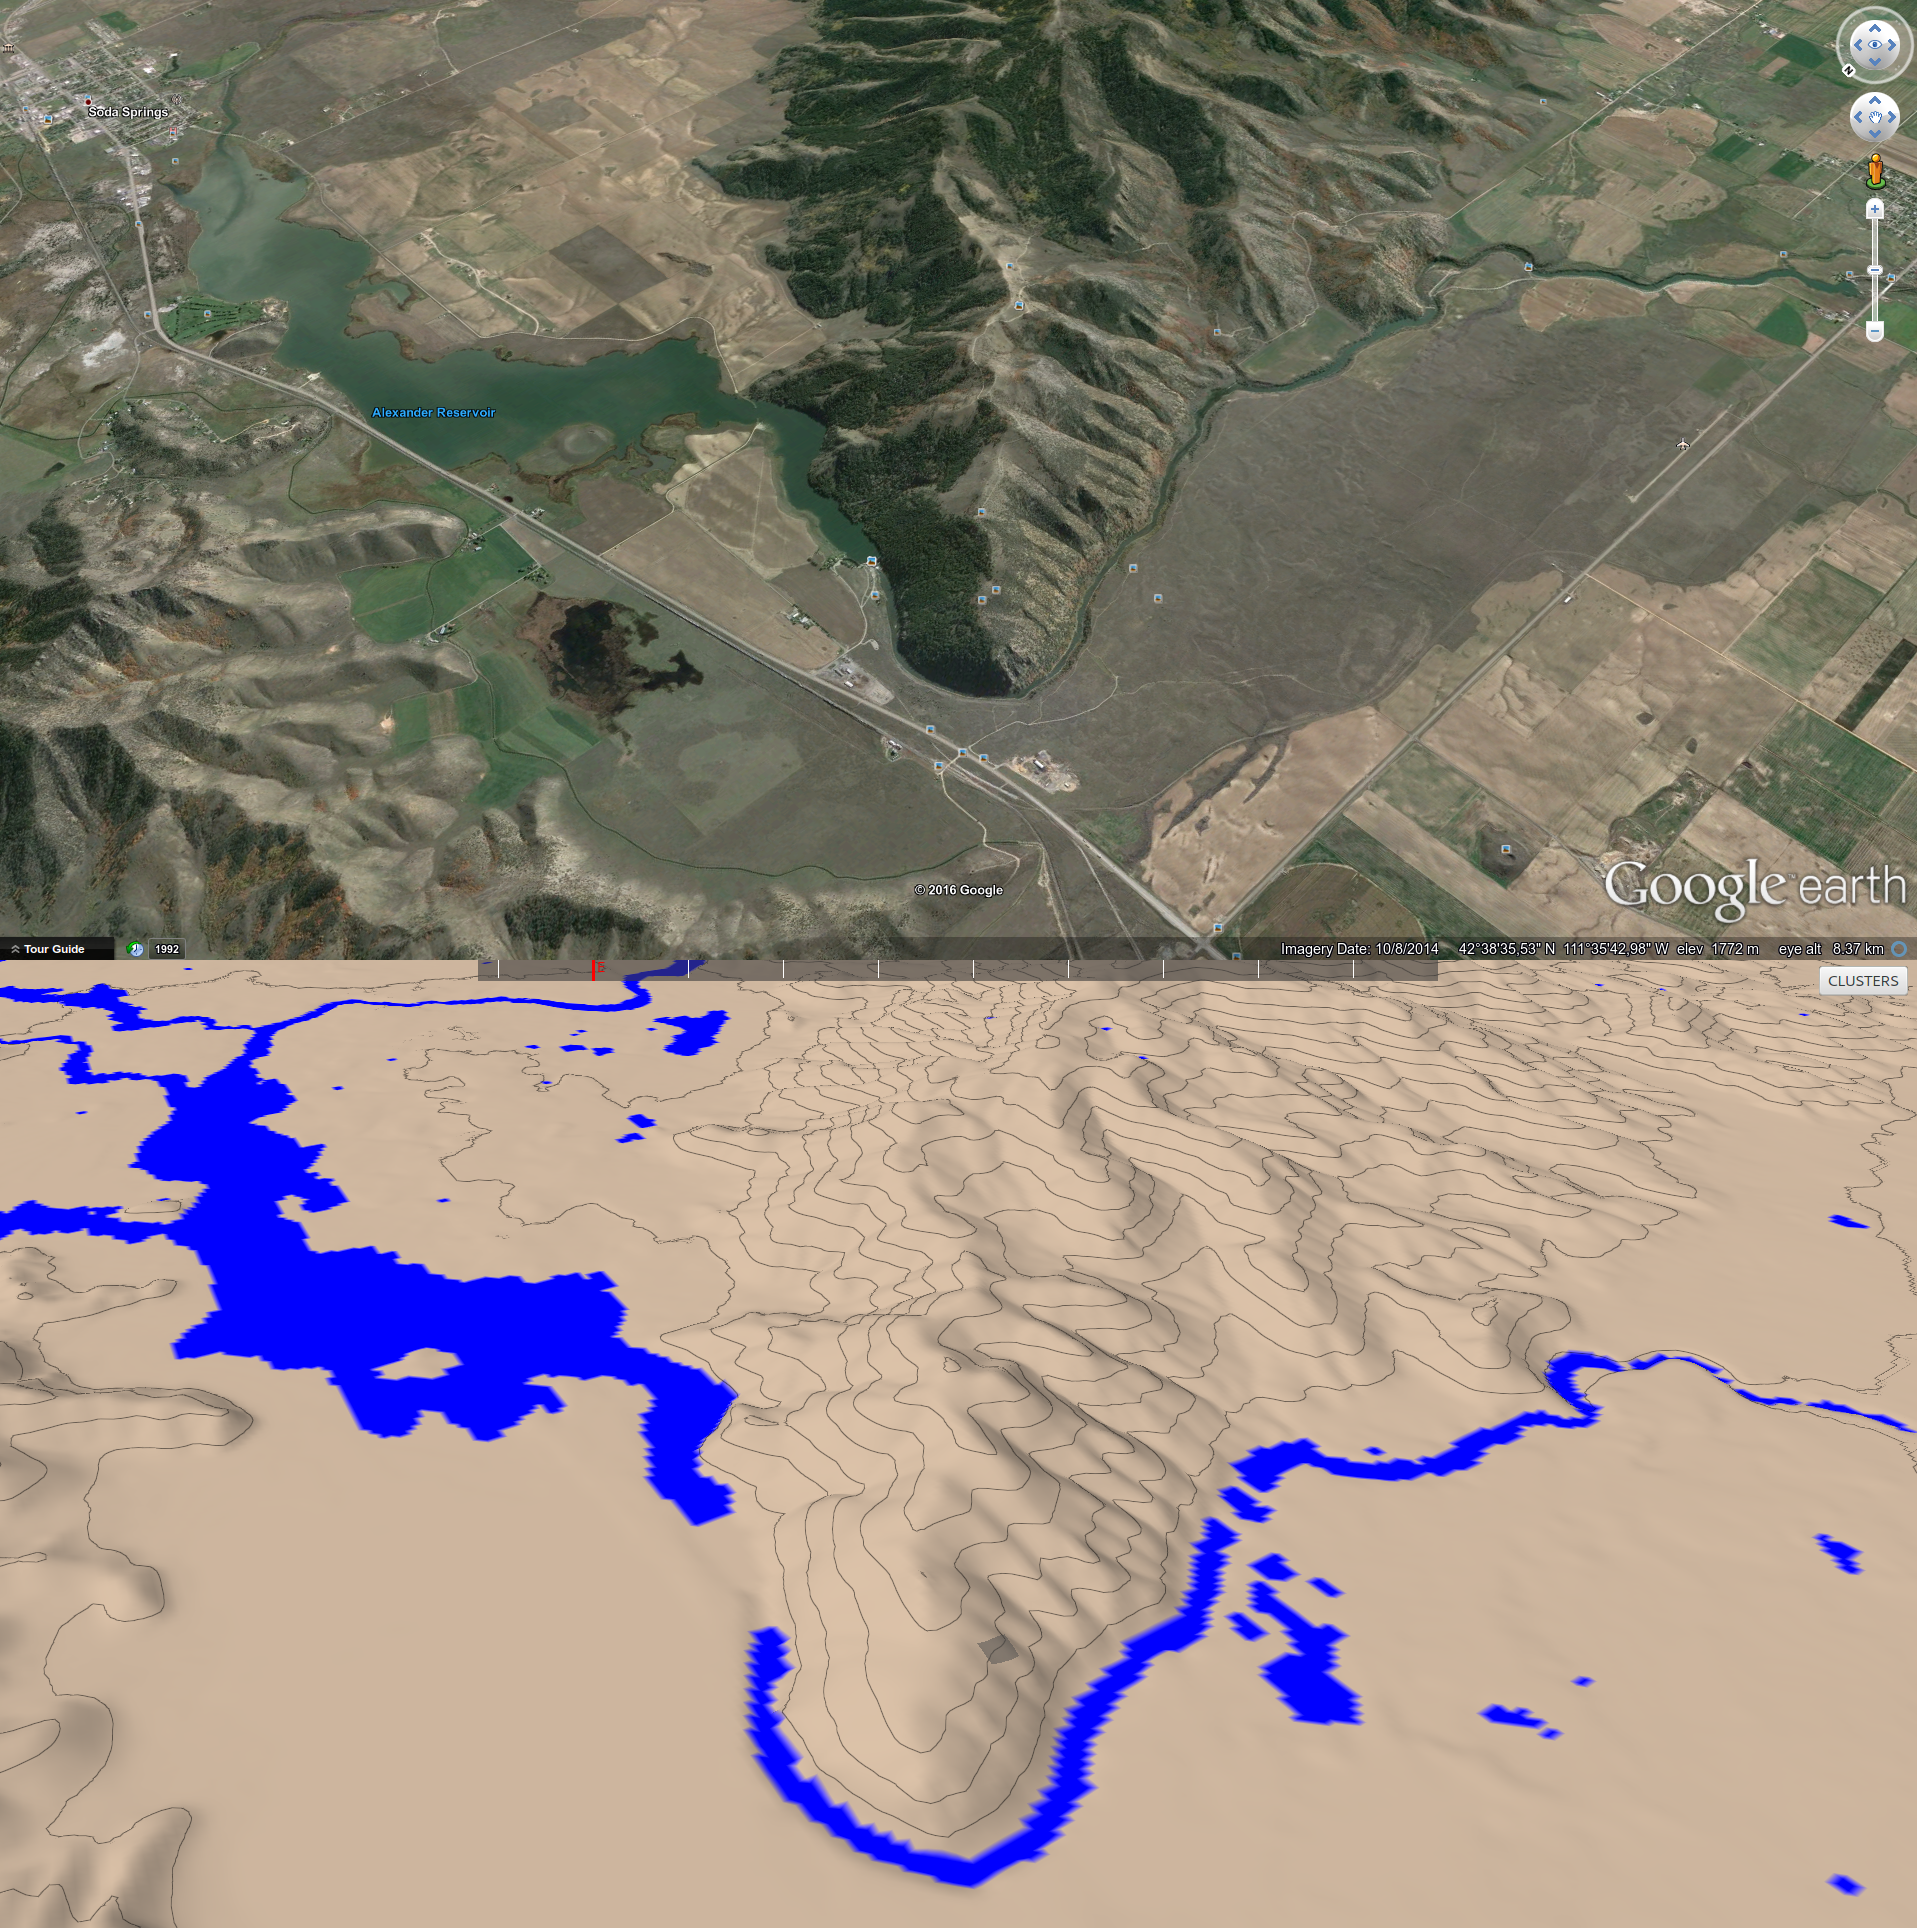
\includegraphics[width=\textwidth]{water_flow_test_1.png}
	\caption{ Top: Real world water-network at geographic coordinate location: 42\textdegree38'N 111\textdegree35'W. Bottom: Replica using the water-flow simulation.}
	\label{fig:water_flow_test_1}
\end{figure}

\begin{figure}
\center
	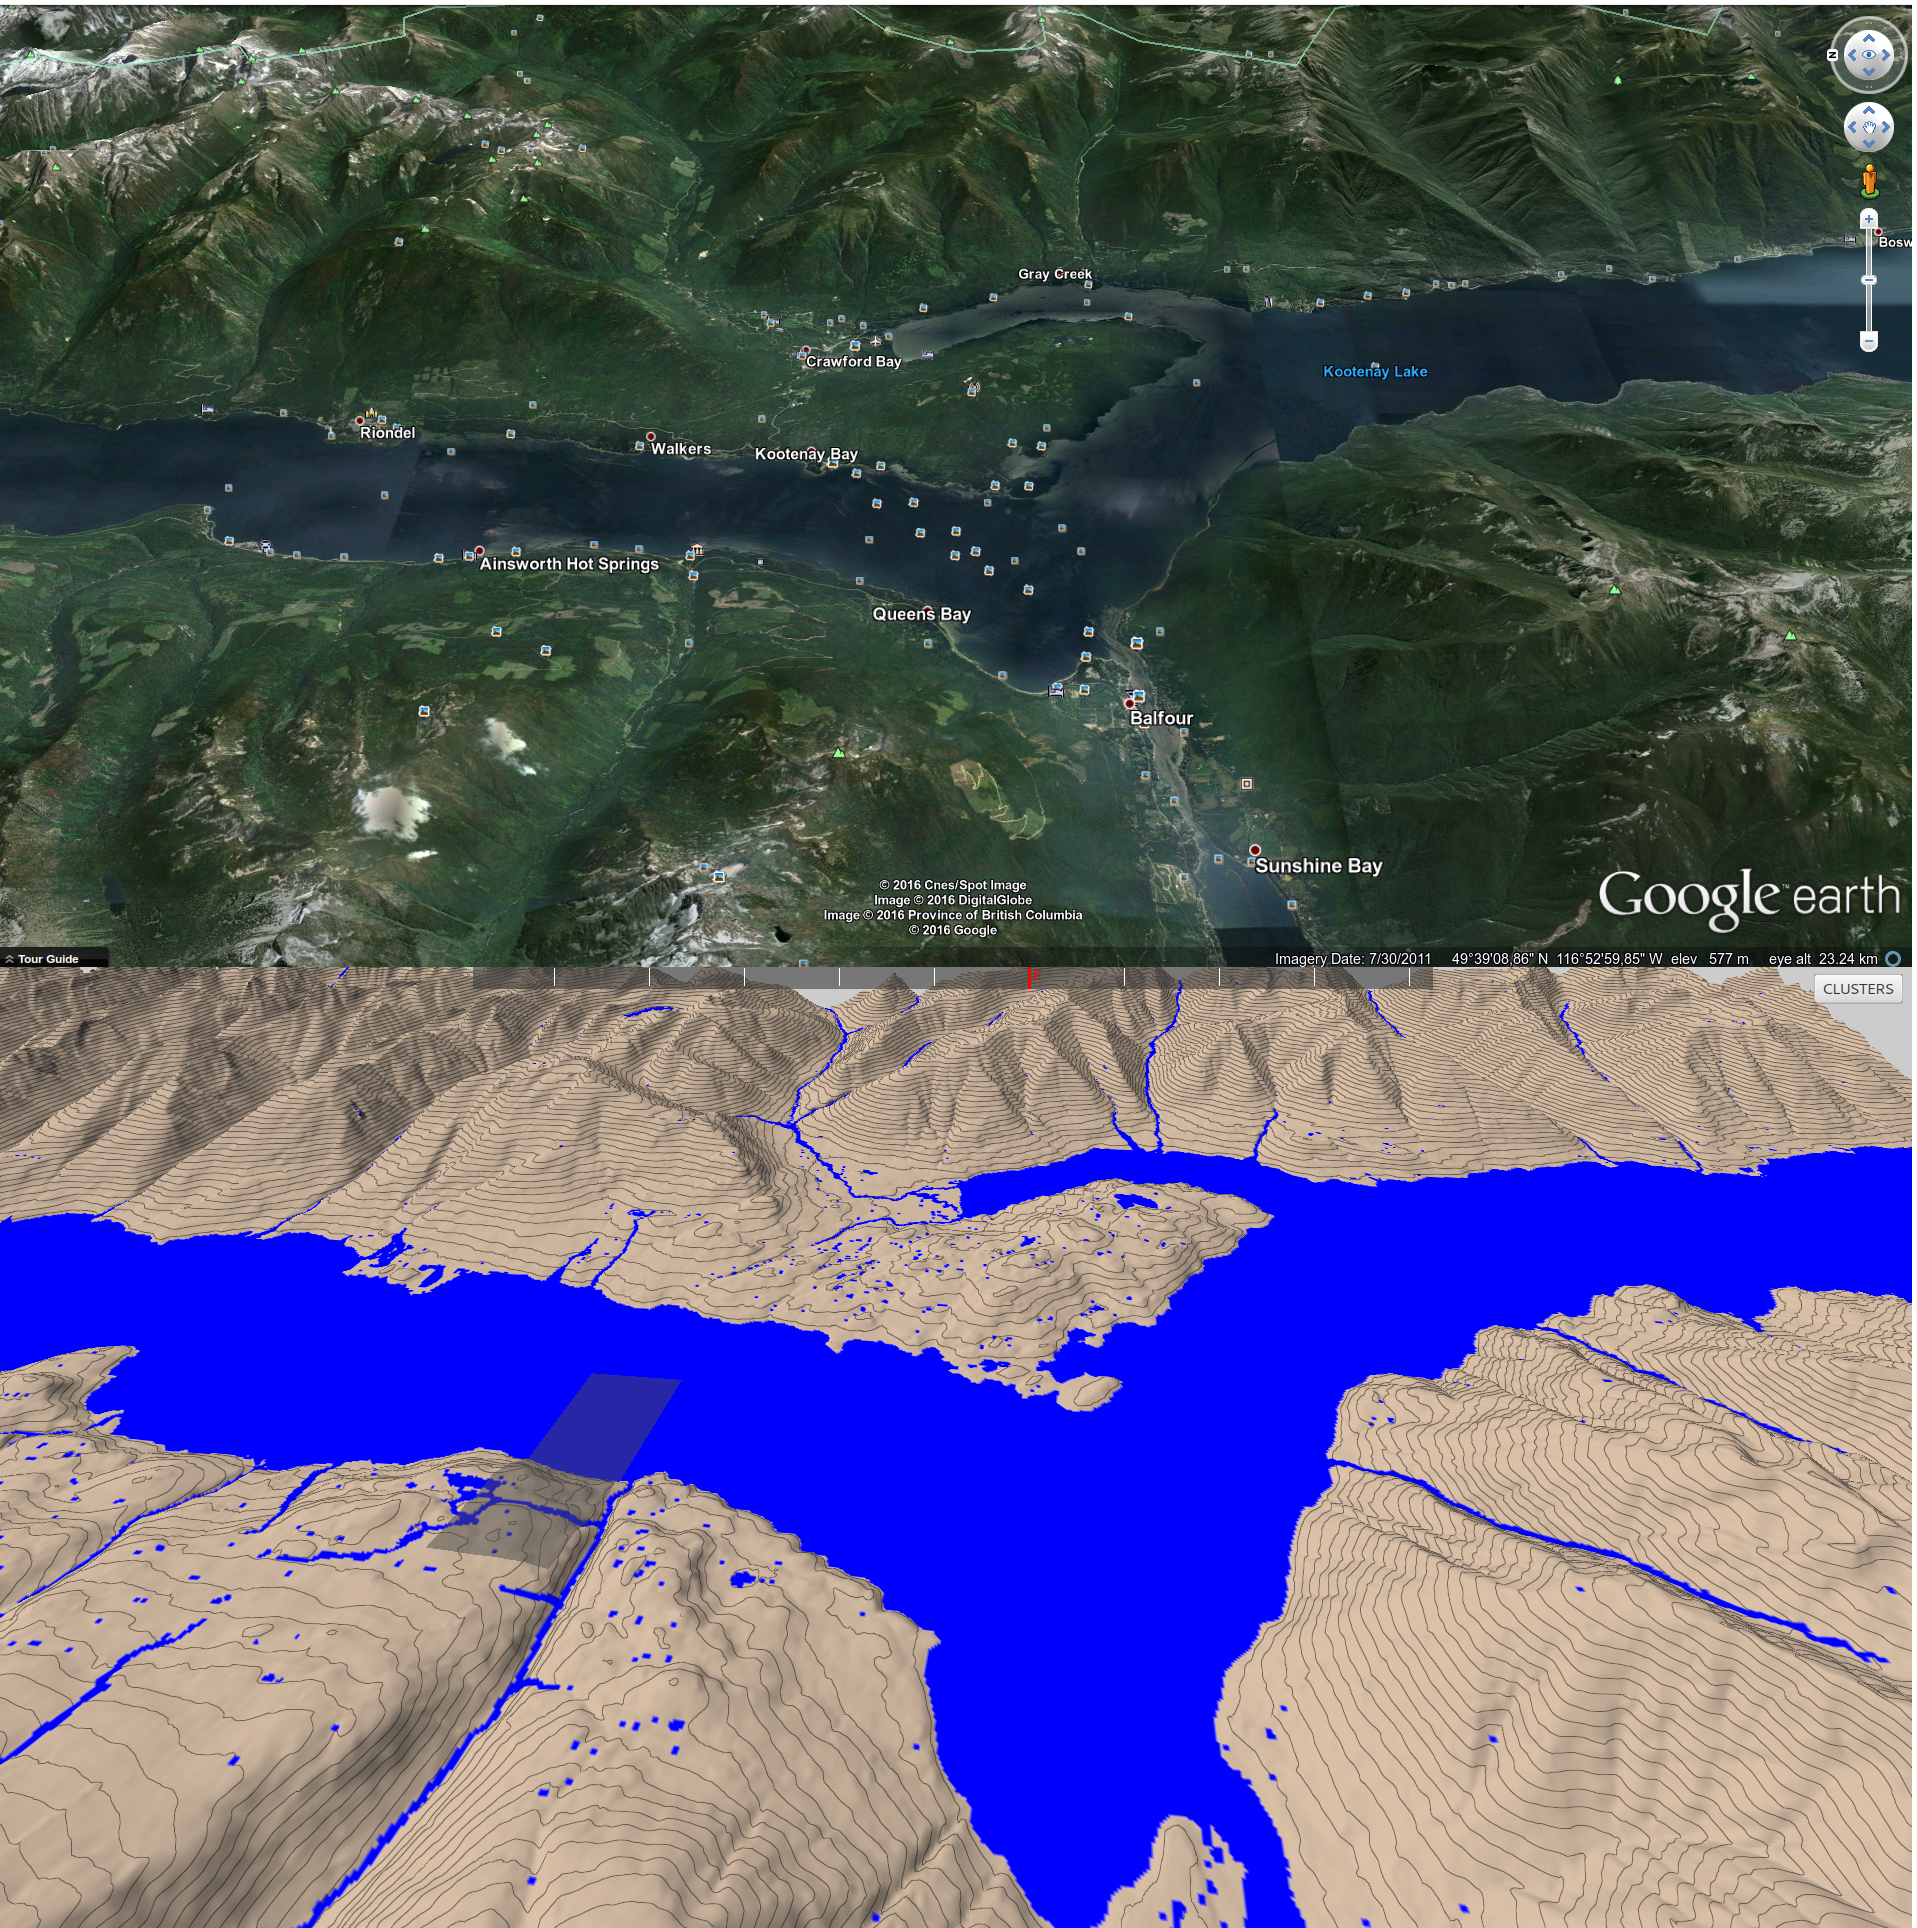
\includegraphics[width=\textwidth]{water_flow_test_2.png}
	\caption{ Top: Real world water-network at geographic coordinate location: 49\textdegree39'N 116\textdegree52'W. Bottom: Replica using the water-flow simulation.}
	\label{fig:water_flow_test_2}
\end{figure}

\begin{figure}
\center
	\includegraphics[width=\textwidth]{water_flow_test_3.png}
	\caption{ Top: Real world water-network at geographic coordinate location: 42\textdegree38'N 111\textdegree35'W. Bottom: Replica using the water-flow simulation.}
	\label{fig:water_flow_test_3}
\end{figure}
\section{Water Bodies}

Water bodies refers here to static water build-ups such as seas, oceans and lakes. The water-flow simulation \label{sec:rivers_and_streams} often fails to reproduce these accurately as they are the result of years of water accumulation, groundwater and different soil infiltration rates. Users can place such water bodies by using a \textit{flood-fill}.

Flood-filling uses a single seed point, \textit{P$_{seed}$}, to determine the height, \textit{H$_{level}$}, at which to set the water-level. This seed point then iteratively propagates to all surrounding points which have height \textit{H} equal or lower than \textit{H$_{level}$} using a flood-fill approach. The process continues until there are no more valid destination points or the terrain extremity is reached. When flood-filling is activated, the user specifies the seed point by simply clicking on it with the mouse pointer. The flood-filling algorithm produces water bodies in real-time even for large terrains and large water-bodies. It is possible to undo an unlimited stack of water body placements added with the flood-filling tool (Ctrl+Z). This is deemed important in case the user mistakenly specifies an incorrect seed point. \\

Figure \ref{fig:flood_fill_test} shows that the tool can be used to successfully place water bodies on the terrain.

\begin{figure}
\center
	\includegraphics[width=\textwidth]{flood_fill_test_ocean.png}
	\caption{ Terrain before (top) and after (top) using the flood-fill tool to place a large water body (e.g sea or ocean). }	
	\label{fig:flood_fill_test}
\end{figure}


\chapter{Clustering}

Each point on the terrain has a number of associated resource properties (summarised in table \ref{tab:point_resources}). These properties are used as input to an ecosystem simulator to determine vegetation and vegetation density. Running an ecosystem simulation for each point on the terrain would be excessive, however, both in terms of computation time and data overlap. The data overlap would be the result of simulations being run for points with very similar resource properties.\\

\begin{table}[h]
  \centering
	    \begin{tabular}{|p{6cm}|p{3cm}|p{6cm}|}
		\hline	
  	    \textbf{Resource} & \textbf{Count} & \textbf{Comments} \\
  	    \hline	
  	    Slope & 1 & - \\
		\hline
  	    Temperature & 12 & Temperature for each month \\
		\hline
  	    Illumination & 12 & Illumination for each month \\
		\hline
  	    Soil Humidity & 12 & Soil humidity for each month \\
		\hline
		\end{tabular}
		\caption{Resource properties associated with a single point on the terrain.}
	  \label{tab:point_resources}
\end{table}

To make the number of ecosystem simulations which need to be run manageable and ensure each one generates distinct distribution data, clustering is performed on the terrain based on the resources of individual points. The type of clustering algorithm used is \textit{K-Means Clustering}, discussed in the dedicated \textit{K-Means Clustering} section. To accelerate the clustering algorithm and strive for real-time results, a GPU implementation was made. Details of which can be found in the \textit{GPU Implementation} section. To conclude the chapter, performance and results are analysed in sections \textit{Performance} and \textit{Results} respectively.


\section{K-Means Clustering} \label{sec:clustering}

K-means is a well known and broadly used vector-quantization clustering algorithm \cite{Jain2010} which groups points into clusters based on the euclidean distance from a set of \textit{K} cluster means. It has been used to to tackle a wide range of problems including character recognition \cite{Perrone2000}, image segmentation \cite{Bradley1998,Kanungo2002} and compression \cite{Kanungo2002}.\\
The algorithm is of complexity O(N) and can be optimized to make use of parallel architectures \cite{Xu2005}. Efficiency is a key requirement for the terrain clustering process in order to provide interactive user feedback, irrespective of terrain size.\\
K-means often fails to produce adequate clusters when dealing with large dimensionality data sets \cite{Sun2012}. Because the data here has only four dimensions (slope, temperature, illumination and soil humidity), it is well-fitted. \\
Common downsides of K-means clustering, however, is the necessity to configure the number of clusters to produce \textit{K} and the selection of the initial \textit{K} points to act as the cluster seeds. How these are handled are discussed in sections \ref{subsec:n_cluster_conf} and \ref{subsec:init_clusters} respectively.\\

Given a set of data points \textit{P} and a configured value \textit{k}, k-means clustering behaves as follows:
\begin{enumerate}
\item Choose \textit{K} points at random to act as the seed cluster means, \textit{C$_{mean}$}.
\item Iterate through every data point \textit{P$_{n}$} from \textit{P} and calculate its Euclidean distance from each cluster mean using equation \ref{eq:cluster_dist_calc}. Point \textit{P} becomes a member of its closest cluster. 
\item Use the members of each cluster to calculate the new cluster means. 
\item Repeat from step 2. 
\end{enumerate}

\begin{equation} \label{eq:cluster_dist_calc}
D(A,B) = \sum_{n=1}^{m} (A_{n} - B_{n}) ^{2}
\end{equation}

Where: \textbf{A} and \textbf{B} are either data points or a cluster mean; \textbf{n} $\in$ \textbf{$\mathbb{R}_{m}$} is the dimensionality of the data set; \textbf{A$_{n}$} is the value of data point A in dimension \textit{n}.

\subsection{Algorithm Complexity}

For each clustering iteration, the algorithm needs to run through each data point twice. The first time, the distance between the data point and each mean cluster is calculated in order to determine the cluster membership.  The second time is to calculate the new cluster means. Given this, the algorithm complexity is $ 2 \times K \ times n \times i$ where: \textit{K} is the number of clusters, \textit{n} is the number of data points and \textit{i} is the total number of clustering iterations performed.

\subsection{Normalisation}

The Euclidean distance calculation outlined in equation \ref{eq:cluster_dist_calc} works well when all values have similar scale. Unfortunately, this is not the case for terrain resource data as illumination, slope, temperature and soil humidity are all measured in different units. This means that a one millimetre change in soil humidity will have as much of an influence on clustering as a one degree change in temperature. To equalise the effect on clustering across all resources, normalisation is performed based on the range of the individual resources. Equation \ref{eq:cluster_dist_calc_real} is used to calculate the Euclidean distance between two terrain positions (or cluster means) \textit{A} and \textit{B} for clustering.

\begin{equation} \label{eq:cluster_dist_calc_real}
D(A,B) = 
(\frac{\textit{S}(A) - \textit{S}(B)}{R_{S}})^{2} + 
\sum_{n=1}^{12}(
(\frac{\textit{T}_{n}(A) - \textit{T}_{n}(B)}{R_{T}}) ^{2} + 
(\frac{\textit{H}_{n}(A) - \textit{H}_{n}(B)}{R_{H}}) ^{2} + 
(\frac{\textit{I}_{n}(A) - \textit{I}_{n}(B)}{R_{I}}) ^{2} )
\end{equation}

Where:\textit{S(x)} is the slope of a point or cluster mean x; \textit{R$_{T}$(x)} is the slope range; ;\textit{T$_{n}$(x)} is the temperature of point or cluster mean x at month n; \textit{R$_{T}$(x)} is the temperature range; \textit{H$_{n}$(x)} is the soil humidity of point or cluster mean x at month n; \textit{R$_{H}$(x)} is the humidity range; \textit{I$_{n}$(x)} is the illumination of point or cluster mean x at month n; \textit{R$_{I}$(x)} is the illumination range; 

\subsection{Configuring the Number of Clusters, K} \label{subsec:n_cluster_conf}

The value of \textit{K} will affect the number of ecosystem simulators which need to be run when placing vegetation on the terrain. Although larger values will potentially result in more realistic vegetation distributions, the added simulations will require additional processing time. Choosing a good value for \textit{K} is therefore about finding a balance between realism and processing time and, as such, depends on user requirements. Too small of a K value will negatively impact realism as insufficient clusters will be generated and terrain vertices will be gathered into a same cluster even if they differ heavily in their underlying resources. Too big a value of K will negatively impact performance as ecosystem simulator runs will be performed to fill distinct areas of the terrain which are heavily similar in terms of the resources they offer. Because of this, the value of \textit{K} is required as input from the user before the clustering is performed.\\
Admitably, \textit{K} can be an abstract to users who don't have an understanding of K-means clustering. Future work could build on this and automatically calculate a suitable value of \textit{K} given the variance of the resources on the terrain.\\

\subsection{Choosing Seed Cluster Means} \label{subsec:init_clusters}

A downside of classic K-means clustering techniques is that clusters are non-reproducible. This is because the final clusters depend heavily on the initial seed points which were chosen to act as the cluster means. As these are selected at random, different runs will result in different clusters. Reproducibility is important here, however, as if the clusters cannot be reproduced neither will the final terrain. To ensure reproducibility, the terrain positions to act as the initial clusters are chosen using a pseudo-random number generator with a predefined and fixed seed.

\section{GPU Implementation}

Performing K-Means clustering is an \textit{O(KN)} problem where K is the number of clusters. As a consequence, given a cluster count, the processing time will increase linearly with terrain area. For large terrains with millions of vertices this could prove time consuming and, consequentially, have a negative effect on user experience. To accelerate the clustering process and maximize user-experience it is implemented to make use of the heavily parallel architecture of the GPU. Below are discussed the details and optimizations of this implementation. \\

\begin{table}[]
  \centering
	    \begin{tabular}{|p{3cm}|p{1.5cm}|p{6cm}|p{5cm}|}
		\hline	
  	    \textbf{Storage Type} &  \textbf{Data Type} & \textbf{Element Count} & \textbf{Usage} \\
		\hline
		3-D Texture & Float & W $\times$ H $\times$ 12 & Monthly Soil Humidity \\
		\hline
		3-D Texture & Float & W $\times$ H $\times$ 12 & Monthly Illumination \\
		\hline
		2-D Texture & Float & W $\times$ H & Temperature \\
		\hline
		2-D Texture & Float & W $\times$ H & Slope \\
		\hline
		3-D Texture & Float & $ \textit{K} \times WorkGroups_{x} \times 13 \times WorkGroups_{y} $ &  Slope and Humidity Reducer \\
		\hline
		3-D Texture & Float & $ \textit{K} \times WorkGroups_{x} \times 2 \times WorkGroups_{y} $ &  Temperature Reducer \\
		\hline
		3-D Texture & Float & $ \textit{K} \times WorkGroups_{x} \times 12 \times WorkGroups_{y} $ & Daily Illumination Reducer \\
		\hline
		\end{tabular}
		\caption{Global memory allocations necessary for the GPU implementation of K-Means clustering. \textit{W} and \textit{H} are the width and height of the terrain respectively. \textit{WorkGroups$_{x}$} and \textit{WorkGroups$_{y}$} are the horizontal and vertical workgroup count respectively.}
	  \label{tab:clustering_mem_allocs}
\end{table}

\subsection{Calculating cluster membership}

Given the cluster means for iteration \textit{i}, the algorithm must determine to which cluster each terrain vertex belongs. To do so efficiently, each GPU core is associated a unique vertex and is responsible for determining it's cluster membership.

\subsection{Calculating the new cluster means}

Once all terrain vertices have been assigned to a cluster, they must be iterated over in order to calculate the new means of each cluster.\\

Within a work-group (group of cores which are guaranteed to run in parallel and have access to shared memory), when each core calculates it's distance from individual cluster means, it loads its associated resource data into a unique index of fast-access shared memory. It also stores in shared memory the calculated cluster membership. This data is then used to calculate, within each work-group, \textit{k} new work-group cluster means, in parallel. The \textit{k} work-group cluster means are then stored to global memory along with the member count for each cluster.\\

Finally, the global cluster means are calculated by \textit{k} cores in parallel using the means calculated for each individual work group along with their associated member counts.\\

\subsection{Storage Optimization}

The temperature on the terrain increases linearly with altitude. As such, even though the temperature changes monthly on the terrain, the temperature difference between two points \textit{P$_{a}$} and \textit{P$_{b}$} will remain constant throughout the year. Calculating the Euclidean distance from a given point \textit{A} to a cluster mean is identical to calculating the difference between two points on the terrain. As a consequence, it is only necessary to use a single months temperature data to establish terrain clusters, saving vital GPU storage space.

\subsection{Minimizing CPU to GPU data transfers}

As mentioned previously, copying data to and from CPU to GPU is a costly process. To prevent these costly transfer operations, all data required for the clustering algorithm (table \ref{tab:clustering_mem_allocs}) is copied to the GPU at the start of the clustering process and no further transfers are performed until completion. \\
\section{Performance}

As mentioned previously, performance is a key requirement for the clustering process. The target is for the clustering to perform in near real-time, irrespective of cluster count or terrain size. This will be put to the test in this section. 


\section{Overlay and Cluster Descriptions}

When clustering is complete, each point on the terrain is associated with one of \textit{k} unique clusters. To make this association apparent to the user a cluster overlay is displayed. The clustering overlay attributes a unique color to each cluster and subsequently each terrain vertex a unique color based on cluster membership (see figure \ref{fig:cluster_overlay}). Along with the terrain overlay, a dialogue shows the properties (color, member count, resources) of each cluster (see figure \ref{fig:cluster_dialog}).

\begin{figure}
\center
	\includegraphics[width=\textwidth]{cluster_overlay.png}
	\caption{ Cluster Overlay. }	
	\label{fig:cluster_overlay}
\end{figure}

\begin{figure}
\center
	\includegraphics[width=\textwidth/2]{cluster_dialog.png}
	\caption{ Cluster properties dialogue. }	
	\label{fig:cluster_dialog}
\end{figure}


\section{Results}

To test the clustering algorithm, a terrain is loaded, it's resources edited and five clusters produced. These clusters are subsequently analysed to ensure they successfully detect distinct resource features on which to cluster.\\

The terrain used is a model of the Grand Canyon using data from the US Geological Survey \protect\footnotemark \footnotetext{\url{http://www.usgs.gov}}. This terrain is chosen as its canyons and crevasses make ground illumination vary greatly.\\

The following resource edits were performed on the terrain:

\begin{itemize}
\item \textit{Latitude}: Set to zero degrees (equator)
\item \textit{Soil Infiltration}: 5 millimetres for all terrain points with a slope under 30 degrees. All points with a slope over 30 degrees were set to 0 to simulate a cliff.
\item \textit{Rainfall}: See table \ref{tab:clustering_test_rainfall}.
\item \textit{Temperature}: 0 degrees at 0 meters in December. 15 degrees at 0 metres in June. Lapse rate at default value of 6.4 degrees per thousand metres.
\end{itemize}

The resulting terrain clusters that form are displayed in figure \ref{fig:clustering_test_resulting_clusters} and summarized in appendix \ref{AppendixA}.

\begin{table}[]
  \centering
	    \begin{tabular}{|p{5cm}|p{5cm}|}
	    \hline
	    \textbf{Month} & \textbf{Rainfall (mm)}\\
		\hline
	    Jan & 13 \\
	    \hline
	    Feb & 15 \\
	    \hline
	    Mar & 14 \\
	    \hline
	    Apr & 9 \\
	    \hline
	    May & 6 \\
	    \hline
	    Jun & 18 \\
	    \hline
	    Jul & 18 \\
	    \hline
	    Aug & 22 \\
	    \hline
	    Sep & 15 \\
	    \hline
	    Oct & 11 \\
	    \hline
	    Nov & 9 \\
	    \hline
	    Dec & 16 \\
	    \hline
		\end{tabular}
		\caption{Monthly rainfall configured for the clustering tests.}
	  \label{tab:clustering_test_rainfall}
\end{table}

\begin{figure}
\center
	\includegraphics[width=\textwidth]{clustering_test_resulting_clusters.png}
	\caption{ \textit{Clustering test: Resulting terrain clusters}}	
	\label{fig:clustering_test_resulting_clusters}
\end{figure}

\begin{figure}
\center
	\includegraphics[width=\textwidth]{clustering_graph_illumination_diff.png}
	\caption{ \textit{Monthly illumination for each cluster and the average over the whole terrain.}}	
	\label{fig:clustering_graph_illumination}
\end{figure}

\begin{figure}
\center
	\includegraphics[width=\textwidth]{clustering_graph_temp_diff.png}
	\caption{ \textit{Monthly temperature for each cluster and the average over the whole terrain. Cluster 2 has the same values as cluster 4.}}	
	\label{fig:clustering_graph_temp}
\end{figure}

\begin{figure}
\center
	\includegraphics[width=\textwidth]{clustering_graph_soil_humidity_diff.png}
	\caption{ \textit{Soil humidity for each cluster (same for every month) and the average over the whole terrain.}}	
	\label{fig:clustering_graph_humidity}
\end{figure}

\begin{table}[]
  \centering
	\begin{tabular}{|p{5cm}|p{5cm}|}
	\hline
	\textbf{Cluster ID} & \textbf{Slope difference (degrees)}\\
	\hline
	1 & -2.5 \\	
	\hline
	2 & 36.7\\	
	\hline
	3 & 59.5\\	
	\hline
	4 & -18\\	
	\hline
	5 & -53.5\\		
	\hline
	\end{tabular}
	\caption{ Difference of slope between the means of each cluster and the terrain mean.}
	\label{tab:clustering_slope_mean}
\end{table}

Figures \ref{fig:clustering_graph_illumination}, \ref{fig:clustering_graph_temp}, \ref{fig:clustering_graph_humidity} and table \ref{tab:clustering_slope_mean} show how much each cluster's illumination, temperature, soil humidity and slope vary from the terrain's average.\\ 

From figure \ref{tab:clustering_test_cluster_variance}, which summarises the resource variance of each cluster, it is possible to identify key terrain features the represent, notably: \textit{Cluster 1} is formed of the data points within the flat bottom of the canyon where the rivers form. Hence the low temperature caused by the low altitude, the low illumination caused by the surrounding canyon walls casting shade, the extremely high humidity caused by the river stream passing through and the flat bottom causing the slope to be very low. \textit{Cluster 2} constitutes the points at the top of the canyon cliffs where slope reduces. Hence the high slope and the low humidity (water run-off). \textit{Cluster 3} contains the data points on the cliffs of the terrain, hence the high slopes, low humidity (water run-off) and low illumination (cliffs often in the shade). \textit{Cluster 4} is formed of the data points most similar to the terrain mean, hence its limited variance. \textit{Cluster 5} is formed of the areas of high altitudes where the surface is flat, illumination is high (nothing to shade it) and temperatures are low.\\

\begin{table}[]
  \centering
	    \begin{tabular}{|p{3cm}|p{3cm}|p{3cm}|p{3cm}|p{3cm}|}
		\hline	
  	    \textbf{Cluster} &  \textbf{Illumination} & \textbf{Temperature} & \textbf{Soil Humidity} & \textbf{Slope} \\
		\hline
		\textbf{1} & 4(-) & 5(+)$^{*}$ & 5(+)$^{*}$ & 1(-) \\
		\hline
		\textbf{2} & 2(-) & 4(+) & 3(-) & 3(+) \\
		\hline
		\textbf{3} & 5(-)$^{*}$ & 2(+) & 4(-)$^{*}$ & 5(+)$^{*}$ \\
		\hline
		\textbf{4} & 1(+) & 1(+) & 1(-) & 2(-) \\
		\hline
		\textbf{5} & 3(+)$^{*}$ & 3(-)$^{*}$ & 2(-) & 4(-)$^{*}$ \\
		\hline
		\end{tabular}
		\caption{Comparison of cluster feature variance from terrain average on a ranking of 1 (least) to 5 (most). The symbol states whether the variance is positive (+) or negative (-). The minimums and maximums for each resource are represented with a $^{*}$. }
	  \label{tab:clustering_test_cluster_variance}
\end{table}

\chapter{Vegetation}

An essential part of rural terrains is vegetation. Available resources determine which plant species are able to grow and to what extent they strive in a given environment. Reproducing this link between species and climate is essential to determine suitable vegetation and subsequently generate plausible terrains. \\

To be able to determine environments suited for given plants, new plants are specified with associated resource requirement properties. Details of which can be found in the \textit{Plant Species} section below.\\
Given these properties, it is possible to automatically filter out ill-suited plants from being suggested to the user. Information about this automatic filtering feature is outlined in the \textit{Resource-based plant filtering} section below.\\

Although a multitude of plants can grow in a given environment, some will naturally strive more than others. This can be because resources are more adequate or they have a faster, more aggressive growth rate. To model this intra-specie battle for resources and  determine a suitable vegetative state, an ecosystem simulator is used. Details of which can be found in the dedicated \textit{Ecosystem Simulator} section below.\\

The ecosystem simulator is computationally expensive and can take some time to determine a valid distribution. The time is dependent on the number of plant instances in the simulation along with the simulation area. To accelerate the process, the ecosystem simulator is run on a small area and the resulting distribution analysed in order to reproduce it on larger area. Information about the distribution analysis and reproduction algorithms can be found in the dedicated \textit{Plant Distribution Analysis and Reproduction} section below.

\section{Plant Species} \label{sec:plant_species}

A database is used to store all plant species and their associated properties, which are used to determine their ability to grow in a given environment and, subsequently, deduce a plausible distribution using the ecosystem simulator. A dedicated tool can be used to interact directly with the database in order to add, remove and edit this data.\\
When configuring a new species it is necessary to specify a set of associated properties. These properties can be split into two main categories: \textit{simulation-based} and \textit{environment-based}. \textit{Simulation-based} properties are those used only by the ecosystem simulator to simulate the growth and spawning of new plants. \textit{Environment-based} properties are those used by the simulator to calculate the strength of the plant but also to determine whether or not it is suited to given environments. Each are discussed below and summarized in table \ref{tab:specie_properties}.\\

\begin{table}[]
  \centering
	    \begin{tabular}{|p{4cm}|p{7cm}|p{2cm}|p{0cm}|}
		\hline	
		\textbf{Property} & \textbf{Value} & \textbf{Units} \\
		\hline
		\multirow{2}{*}{\textbf{Slope}} & \multicolumn{1}{l|}{Start of decline} & \multicolumn{1}{l|}{Degrees} \\\cline{2-3}
        						   & \multicolumn{1}{l|}{Maximum} & \multicolumn{1}{l|}{Degrees} \\
		\hline
		\multirow{3}{*}{\textbf{Growth}} & \multicolumn{1}{l|}{Maximum canopy} & \multicolumn{1}{l|}{Centimetres} \\\cline{2-3}
        						   & \multicolumn{1}{l|}{Maximum root size} & \multicolumn{1}{l|}{Centimetres} \\\cline{2-3}
                               & \multicolumn{1}{l|}{Maximum height} & \multicolumn{1}{l|}{Centimetres} \\
		\hline
		\multirow{2}{*}{\textbf{Ageing}} & \multicolumn{1}{l|}{Start of decline} & \multicolumn{1}{l|}{Months} \\\cline{2-3}
        						   & \multicolumn{1}{l|}{Maximum age} & \multicolumn{1}{l|}{Months} \\
		\hline    
		\multirow{2}{*}{\textbf{Seeding}} & \multicolumn{1}{l|}{Maximum seeding distance} & \multicolumn{1}{l|}{Metres} \\\cline{2-3}
        						   & \multicolumn{1}{l|}{Annual seed count} & \multicolumn{1}{l|}{ - } \\
		\hline    
		\multirow{4}{*}{\textbf{Illumination}}
								& \multicolumn{1}{l|}{Start of prime} & \multicolumn{1}{l|}{hours} \\\cline{2-3}
								& \multicolumn{1}{l|}{End of prime} & \multicolumn{1}{l|}{hours} \\\cline{2-3}
								& \multicolumn{1}{l|}{Minimum} & \multicolumn{1}{l|}{hours} \\\cline{2-3}
								& \multicolumn{1}{l|}{Maximum} & \multicolumn{1}{l|}{hours} \\
		\hline   
		\multirow{4}{*}{\textbf{Humidity}}
								& \multicolumn{1}{l|}{Start of prime} & \multicolumn{1}{l|}{millimetres} \\\cline{2-3}
								& \multicolumn{1}{l|}{End of prime} & \multicolumn{1}{l|}{millimetres} \\\cline{2-3}
								& \multicolumn{1}{l|}{Minimum} & \multicolumn{1}{l|}{millimetres} \\\cline{2-3}
								& \multicolumn{1}{l|}{Maximum} & \multicolumn{1}{l|}{millimetres} \\
		\hline    
		\multirow{4}{*}{\textbf{Temperature}}
								& \multicolumn{1}{l|}{Start of prime} & \multicolumn{1}{l|}{degrees} \\\cline{2-3}
								& \multicolumn{1}{l|}{End of prime} & \multicolumn{1}{l|}{degrees} \\\cline{2-3}
								& \multicolumn{1}{l|}{Minimum} & \multicolumn{1}{l|}{degrees} \\\cline{2-3}
								& \multicolumn{1}{l|}{Maximum} & \multicolumn{1}{l|}{degrees} \\
		\hline                                                                           
		\end{tabular}
	\label{tab:specie_properties}	
	\caption{Summary of the properties which must be configured with each plant species.}
\end{table}

\subsection{Simulation-based Species Properties}

%Growth
To model the growth of a plant species in the ecosystem simulator, it is necessary to specify: \textit{Maximum height}, \textit{maximum canopy width} and \textit{maximum root size}. Using these along with the specie's ageing properties, it is possible to simulate the plants vertical growth (height), horizontal growth (canopy) and root coverage. A plants height and canopy width is also used to determine the shade it projects on other plants during the simulation. Furthermore, the plant's root growth is used to determine how far the plant can reach to fetch soil water. Note that a maximum canopy width of zero can be specified to model plants with no canopy.\\

%Ageing
Biological life-cycle varies greatly between plant species. Whereas annual and biennials have a fixed lifespan of one and two years, respectively, perennial plant species can live far longer. To model the life-cycle of different plant species they must be configured with an associated \textit{age of start of decline} and \textit{maximum age}. Using these two values, it is possible to simulate a plant getting weaker and, therefore, becoming more susceptible to domination from surrounding plants.\\

%Seeding
It is necessary to replicate the spawning of offspring in the ecosystem simulator for two core reasons: \textit{Propagation}: Plants propagate on a terrain by producing new offspring which attempt to spawn and invade different areas. \textit{Succession}: New plants spawn to later succeed older and weaker plants of the same specie.\\ 
The two most common ways for plants to spawn new offspring is through sexual and asexual reproduction. Asexual reproducing species often spawn cloned offspring through budding (e.g potato). Sexual reproducing species, on the other hand, require chromosome exchange between males and females in order to produce unique offspring often propagated via seeds or spores. Although biologically different, both can be considered identical for the sole purpose of modelling propagation and succession. The reproduction characteristics of a given specie which will influence \textit{propagation} and \textit{succession} in the simulation and therefore need to be configured, are the \textit{number of offspring produced annually} and the \textit{maximum distance from source to offspring}.\\

\subsection{Environment-based Species Properties}

%SLOPE
Steep slopes causes essential water and soil nutrients to run-off, making them less rich and, therefore, less suited to plant growth \cite{Kapolka2010}. The slope angle can also cause larger species to struggle in supporting their own biomass. For this reason, steeper slopes often cater better to smaller plant species (grass, shrub, etc.). To model the effect of slope on given plant species, when configuring a new plant species, the \textit{slope of start of decline} and \textit{maximum slope} must be configured.\\

%Illumination
Illumination, soil humidity and temperature also have a great impact on plant growth and survival \cite{Fourcaud2008}.\\
Whereas some species thrive in shaded undergrowth, others require direct illumination all year round. Soil water deposited into the soil by either rainfall or existing groundwater is absorbed by plant roots and is vital to their development and survival. Some species have evolved to survive in arid climates with very little water, others require frequent downpours of rain. To simplify water requirement specifications for different plant species, we ignore groundwater and consider rainfall as the plants only source of water. Some species are able to withstand extremely low temperatures (e.g at high altitudes), others have the ability to survive in extremely hot temperatures (e.g deserts).\\
To configure the illumination, soil humidity and temperature requirements of a given species, it is necessary to configure for each the \textit{minimum}, \textit{prime range} and \textit{maximum}. The minimum represents the minimum illumination (hours), soil humidity (millimetres) or temperature (degrees) necessary for the species survival, the prime range are the values at which the resource is deemed optimal and the maximum is the upper limit after which the plant is unable to survive.


\section{Plant Suitability Filtering} \label{sec:plant_suitability_filtering}

Once the terrain clusters have been generated, the user must specify the plant species to incorporate. The ecosystem simulator is then used to determine a suitable distribution for the species given the resources associated with the individual clusters.\\

Rather than permit the user to select any plant from the database, including those unable to grow, a filtering pass is performed in order to display only the plants best able to survive. This is useful as it prevents users from triggering an ecosystem simulation run with species that are guaranteed not to survive. To determine whether a given species is suited, a \textit{species suitability score} is calculated for each species based on the resources of each cluster. \\

As well as being used to filter out ill-suited species, this suitability score also highlights the species best suited to the given environment and could, as a consequence, prove to be useful information for the user when selecting plant species. Various methods are used to effectively communicate the suitability score, details of which are discussed below.

\subsection{Calculating the Species Suitability Score}

The species suitability score associated with a given species, \textit{S}, for cluster \textit{C}, illustrates how suited species \textit{S} is to the environment of cluster \textit{C} on a range from 0 (completely ill-suited) to 100 (perfect conditions). To calculate this, the resource requirements of species \textit{S} are matched with the resource availability of cluster \textit{C}. To determine this score, it is first necessary to determine the specie's suitability to the environment in terms of \textit{slope}, \textit{illumination}, \textit{soil humidity} and \textit{temperature}. A separate score is calculated for each as discussed below. Note that no filtering is based on illumination as it varies during the simulation as the canopy of taller plants shade that of the smaller ones.\\

The slope suitability score determines how well suited the species is in terms of slope and is calculated as illustrated in equation \ref{eq:slope_suitability_score}.\\

\begin{equation}
\centering
SS(S,x) = 
\begin{cases}
    100, & \text{if } x \leq S_{sod} \\
    0, & \text{if } x \geq S_{max} \\
	(1-\frac{x-S_{sod}}{S_{max}-S_{sod}}) \times 100, & \text{otherwise}
\end{cases}
\label{eq:slope_suitability_score}
\end{equation}
Where: \textit{SS(S,x)} is the slope suitability score for species \textit{S} given slope \textit{x}; \textit{S$_{sod}$} is slope of start of decline configured for species \textit{S}; \textit{S$_{max}$} is the maximum slope configured for species \textit{S}.

Because the soil humidity and temperature vary on a monthly basis, it is necessary to calculate the score for each month as illustrated in equation \ref{eq:monthly_score}. The mean of these twelve months is then calculated as illustrated in equation \ref{eq:avg_score} to represent the overall suitability score for the given resource.

\begin{equation}
\centering
MRS(S,r,x) = 
\begin{cases}
    0, & \text{if } x < S_{min}(r) \text{ or } x > S_{max}(r) \\
    \frac{x - S_{min}(r)}{S_{ps}(r) - S_{min}(r)} \times 100, & \text{if } x \in [S_{min}(R),S_{ps}(R)] \\
    100, & \text{if } x \in [S_{prime_start}(r),S_{prime_end}(r)] \\
    (1 - \frac{x - S_{pe}(r)}{S_{max}(r)-S_{pe}(r)}) \times 100, & \text{if } x \in [S_{pe}(r),S_{max}(r)] \\
\end{cases}
\label{eq:monthly_score}
\end{equation}
Where: \textit{MRS(S,r,x)} is the monthly suitability score for species \textit{S} and resource \textit{r} given resource value \textit{x} at the given month; \textit{S$_{min}$(r)} is the minimum configured for species \textit{S} and resource \textit{r};\textit{S$_{max}$(r)} is the maximum configured for species \textit{S} and resource \textit{r}; \textit{S$_{ps}$(r)} and \textit{S$_{pe}$(r)} constitute the start and end of the prime range configured for species \textit{S} and resource \textit{r}, respectively.\\

\begin{equation}
\centering
RSS(S,r) =
\begin{cases}
	\frac{\sum_{m=1}^{m=12} MRS(S,r,value(r,m))}{12}, & \text{if } MRS(S,R,rv(m)) > 0 \text{ for } m \in [1,12] \\
    0,              & \text{otherwise}
\end{cases}
\label{eq:avg_score}
\end{equation}
Where: \textit{RSS(S,r)} is the resource suitability score for species \textit{S} and resource \textit{r}; \textit{value(r,m)} is the value of resource \textit{r} at month \textit{m}; \textit{MRS(S,r,rv)} is the monthly resource score for species \textit{S}, resource \textit{r} and resource value \textit{rv} (see equation \ref{eq:monthly_score});\\

The overall suitability score gives an overview of the species suitability to the environment for all resources and is calculated as described in equation \ref{eq:specie_suitability_score}

\begin{equation}
\begin{split}
\centering
OSS(S,sl) = 
\begin{cases}
	\frac{SS(S,sl) + \sum_{r}^{}RSS(S,r)}{4} \text{ for } r \in ITS, & \text{if } SS(sl) > 0 \text{ and } RSS(S,r) > 0 \text{ for } r \in ITS \\
	0, &\text{ otherwise} \\
\end{cases}
\end{split}
\label{eq:specie_suitability_score}
\end{equation}
Where: \textit{OSS(S)} is the overall suitability score for species \textit{S}; \textit{AR} = \{temperature,soil humdity \}; \textit{RSS(S,r)} is the resource suitability score for species \textit{S} and resource \textit{r} (see equation \ref{eq:avg_score}); \textit{SS(S,sl)} is the slope suitability score for species \textit{S} given slope \textit{sl} (see equation \ref{eq:slope_suitability_score}); 

\subsection{Communicating the Species Suitability Score}

When all the terrain clusters have been created, the terrain suitability score for each species in the plant database is calculated in relation to the resources of each individual cluster. If the calculated score is zero for all clusters, the species is automatically filtered out to prevent the user from selecting it. \\

To further communicate this information, selectable species are sorted in descending order of their overall species suitability score. Colour coding is also used where each species is associated with a colour ranging from red (very ill-suited) to light green (completely suited).\\

When the user selects a given species, all intermediate scores which were used to calculate the \textit{species suitability score} are communicated to the user in histogram form (see figure \ref{fig:specie_intermediate_suitability_scores}).

\begin{figure}
\center
	\includegraphics[width=\textwidth]{specie_suitability_temp_and_avg.png}
	\caption{ \textit{Overall (top) and temperature (bottom) intermediate species suitability histograms. Not displayed but also is the humidity intermediate species suitability histograms.}}	
	\label{fig:specie_intermediate_suitability_scores}
\end{figure}



\section{Ecosystem Simulator}

Once the user selects the union of all species that must appear in all clusters of the terrain, it is necessary to determine a valid vegetation distribution for each cluster. To do so, an ecosystem simulator is used similarly to that in the work by Deussen et al \cite{Deussen1998} and Lane and Przemyslaw \cite{Lane2002}. Unlike these other ecosystem simulators, however, it isn't based on L-Systems and models both resource requirements and resource availability in greater detail. The purpose of ecosystem simulator is to determine, given a vegetative state, \textit{S$_{t}$} at time \textit{t}, the vegetative state \textit{S$_{t+n}$} at time \textit{t+n}, for any value of n.  \\

To do so, the simulation advances through time in monthly intervals and the strength of all plant instances are re-calculated at each iteration. Their strength depend not only on resource properties of the given month but also surrounding plants as they battle for these resources. Determining the set S = \{P$_{1}$, P$_{2}$, P$_{3}$, ...\} of plants which compete for resources with plant \textit{P$_{n}$} depends on the spatial reach of \textit{P$_{n}$}. Spatial awareness is therefore a key requirement of the simulation which is achieved by splitting the simulation area into a grid of cells as described in \textit{Gridded Simulation Area}.\\

Within each cell of the gridded simulation area, resources must be distributed to the different plant instances present. How this is done is described in \textit{Resource Distribution}. \\

Given the resources allocated to each plant instance, it is possible to calculate their strength. This is used as a representation of the plant's health and, consequentially, it's ability to survive and grow. Details about the plant's strength calculation and it's usage are discussed in \textit{Plant Strength Calculation} and \textit{Plant Strength Usage} respectively.\\

On an annual basis, new plant instances are spawned based on the specie's seeding properties. How this is done is discussed in \textit{Spawning Plants}.\\

To conclude the discussion on the ecosystem simulator, performance and results will be analysed and discussed.

\subsection{Gridded Simulation Area}

The simulation window greatly effects the performance of the ecosystem simulator and, therefore, it is necessary to keep it to a minimum. However, too small a simulation area will fail to accurately model the interaction of larger plant species. Given these constraints, a simulation window of one hundred by one hundred meters is used, accurate to the nearest centimetre. To model plant's interacting and battling for resources, the window is split into cells to form a grid as illustrated in figure \ref{fig:simulation_grid}.\\

\begin{figure}
\center
	\includegraphics[width=\textwidth/2]{simulation_grid.png}
	\caption{ Gridded simulation area.}	
	\label{fig:simulation_grid}
\end{figure}

The size of individual cells can be configured to increase/decrease the resolution and, therefore, the accuracy of the simulation. As the simulation progresses, plant's grow, their spatial coverage increases, and they enter new grid cells. When a plant enters a new grid cell, it becomes a member of it and cell resources must be distributed to it as well as to all other plants in the cell. The information associated to each individual grid cell can be split into two categories: \textit{time-dependent} and \textit{simulation-dependent}. The time-dependent information depends only on the current month, is identical for every grid cell and is comprised of: the \textit{soil humidity} and the \textit{illumination}. The simulation-dependent information changes throughout the simulation as plants spawn, die and grow and is comprised of: the list of plants whose roots intersect the cell and the list of plants whose canopy intersects the cell.

\subsection{Resource Distribution}

The strength of each plant in the simulation must be recalculated on a monthly basis. To determine the strength of a given plant, it is necessary to know the illumination and humidity allocated to it along with the temperature. The temperature is not a distributable resource and is identical for all plant instances given the month. The allocated humidity and illumination is determined by averaging the resources distributed to it in each cell it overlaps in the grid. So, before the strengths of individual plant instances can be calculated, first each cell of the grid must be iterated over and illumination and humidity distributed to the plants contained within. How these are allocated is discussed below.

\subsubsection{Humidity Distribution}

Plants grow there roots in order to access the nutrients and moisture available in the surrounding soil. As roots of different plants overlap, they start to compete for these resources.\\

When distributing the soil humidity of a given grid cell \textit{C$_{xy}$} to the set \textit{S} = \{P$_{1}$, P$_{2}$, P$_{3}$, ...\} of plants which roots intersect the cell, one of three distinct scenarios can occur depending on the total available humidity of the cell: \textit{Abundant humidity}, \textit{sufficient humidity} and \textit{insufficient humidity}.\\

The humidity is deemed abundant if the available humidity, \textit{H$_{available}$}, surpasses 300 millimetres. In this situation, the humidity is deemed to be enough for there to be standing water and therefore all plants of \textit{S} are allocated \textit{H$_{available}$}. \\

If \textit{H$_{available}$} is less than 300 millimetres, it is necessary to determine whether the humidity is sufficient or insufficient by calculating the requested humidity \textit{H$_{requested}$} as outlined in equation \ref{eq:humidity_requested_calc}. 

\begin{equation}
H_{requested} = \sum MinHumidity(P_{n}) \text{ for } n \in S
\label{eq:humidity_requested_calc}
\end{equation}
Where:\textit{MinHumidity(P$_{n}$)} is the minimum humidity requirement of the specie to which plant \textit{P$_{n}$} belongs;\textit{S} is the set of plants whose roots intersect with the given grid cell.

If \textit{H$_{requested}$} is less than \textit{H$_{available}$}, the humidity is deemed sufficient and the amount allocated to each plant is calculated as described in equation \ref{eq:humidity_allocation_sufficient_calc}. If \textit{H$_{requested}$} is more than \textit{H$_{available}$}, however, the humidity is deemed insufficient and the allocation is done following equation \ref{eq:humidity_allocation_insufficient_calc}

\begin{equation}
\begin{split}
H_{allocated}(P_{n}) = MinHumidity(P_{n}) + OverFlow \\
OverFlow = H_{available} - \sum MinHumidity(P_{n}) \text{ for } n \in S
\end{split}
\label{eq:humidity_allocation_sufficient_calc}
\end{equation}
Where:\textit{H$_{allocated}$(P$_{n}$)} is the humidity allocated to plant \textit{P$_{n}$}; \textit{MinHumidity(P$_{n}$)} is the minimum humidity requirement of the specie to which plant \textit{P$_{n}$} belongs;\textit{S} is the set of plants whose roots intersect with the given grid cell.

Intuitively, it allocates each plant with the minimum amount of humidity it requires to survive plus the resulting overflow.

\begin{equation}
\begin{split}
H_{allocated}(P_{n}) = min(MinHumidity(P_{n}), Vigor(P_{n}) \times H_{remaining}) \\
Vigour(P_{n}) =  \frac{RootSize(P_{n})}{\sum RootSize(P_{x}) \text{ for } x \in S}\\
H_{remaining} = H_{available} - (\sum H_{allocated}(P_{x})  \text{ for } x \in S_{processed})\\
\end{split}
\label{eq:humidity_allocation_insufficient_calc}
\end{equation}
Where: The plants of \textit{S} \textbf{must} be iterated over in decrementing order of their vigor as this will affect the water they are allocated; \textit{H$_{allocated}$(P$_{n}$)} is the humidity allocated to plant \textit{P$_{n}$}; \textit{MinHumidity(P$_{n}$)} is the minimum humidity requirement of the specie to which plant \textit{P$_{n}$} belongs; \textit{Vigour(P$_{n}$)} is the vigor of plant \textit{P$_{n}$} in comparison to other plants present in the cell. It is estimated based on root size; \textit{RootSize(P$_{n}$)} is the root size of plant \textit{P$_{n}$}; S$_{processed}$) is the set of plants from \textit{S} whose water allocation has already been calculated; \textit{S} is the set of plants whose roots intersect with the given grid cell.

Intuitively, this algorithm prioritises water distribution to more vigorous plant's.

\subsubsection{Plant Humidity Allocation}

To calculate the humidity allocated to plant \textit{P$_{n}$}, it is first necessary to determine the set of grid cells \textit{S} = \{C$_{1}$, C$_{2}$, C$_{3}$, ...\} which it's roots intersect. Given this, the plants humidity allocation is calculated using equation \ref{eq:plant_humidity_allocation}. 

\begin{equation}
H_{n} = \frac{\sum H_{allocated}(C_{x}) \text{ for } x \in S}{| S |}
\label{eq:plant_humidity_allocation}
\end{equation}
Where:\textit{H$_{n}$} is the humidity allocated to plant \textit{P$_{n}$}; \textit{H$_{allocated}$(C$_{n}$)} is the humidity allocated to plant \textit{P$_{n}$} in grid cell C$_{n}$; \textit{$|$ S $|$} is the number of cells in the set \textit{S}.

Intuitively, the humidity allocated to a given plant is simply the average of the humidity allocated to it in all grid cells it's roots intersect.

\subsubsection{Illumination Distribution}

Plants which are heavily dependent on illumination will often grow a large canopy in order to maximize the leaf area receiving direct sunlight. Doing so also restricts the illumination received by smaller plants in the undergrowth. To model the shade projection of larger plants, illumination is distributed in each cell depending on the plants height and canopy width.\\

Equation \ref{eq:illum_distribution} is used to allocate illumination amongst the set \textit{S} = \{P$_{1}$, P$_{2}$, P$_{3}$, ...\} of plants which canopy intersects cell \textit{C$_{xy}$}.

\begin{equation}
\centering
Illumination(P_{n}) = 
\begin{cases}
	C_{illumination}, & \text{if } CanopyWidth(P_{n}) = 0 for x \in S \\
	C_{illumination}, & \text{if } Height(P_{n}) > height(x) for x \in S : x \neq P_{n} \\
    0,              & \text{otherwise}
\end{cases}
\label{eq:illum_distribution}
\end{equation}
Where: \textit{Illumination($P_{n}$)} is the illumination allocated to plant \textit{P$_{n}$} whose canopy overlaps with current grid cell;\textit{C$_{illumination}$} is the monthly illumination of the cell;\textit{CanopyWidth(P$_{n}$)} is the canopy width of plant P$_{n}$; \textit{Height(P$_{n}$)} is the height of plant P$_{n}$; \textit{S} is the set of plants whose canopy intersects with the given grid cell.

Intuitively, if all plants present in the given cell are canopy-free (i.e no shade projection), the equation allocates them all the available illumination. If not all plants are canopy-free, the equation allocates illumination only to the tallest canopy plant.

\subsubsection{Plant Illumination Allocation}

Calculating the illumination allocated to a plant \textit{P$_{n}$} is very similar to calculating the humidity allocation only the set of grid cells \textit{S} = \{C$_{1}$, C$_{2}$, C$_{3}$, ...\} are those which the plants canopy intersects. Given \textit{S}, the plant illumination is calculated using equation \ref{eq:plant_illumination_allocation}.

\begin{equation}
I_{n} = \frac{\sum I_{allocated}(C_{x}) \text{ for } x \in S}{| S |}
\label{eq:plant_illumination_allocation}
\end{equation}
Where:\textit{I$_{n}$} is the illumination allocated to plant \textit{P$_{n}$}; \textit{I$_{allocated}$(C$_{n}$)} is the illumination allocated to plant \textit{P$_{n}$} in grid cell C$_{n}$; \textit{$|$ S $|$ } is the number of cells in the set \textit{S}.
\end{itemize}

Intuitively, the illumination allocated to a given plant is simply the average of the humidity allocated to it in all grid cells it's canopy intersect.

\subsection{Plant Strength Calculation}

The strength of plant \textit{P$_{n}$} is the minimum of \textit{S$_{age}$}, \textit{S$_{temperature}$}, \textit{S$_{illumination}$} and \textit{S$_{humidity}$} which represent the strength of the plant in terms of it's age, temperature, illumination and humidity respectively. To calculate these values, ranging from negative to positive one hundred, a graph is plotted for each specie based on it's properties as outlined in figures \ref{fig:strength_calc_age}, \ref{fig:strength_calc_temp}, \ref{fig:strength_calc_temp}, \ref{fig:illumination_strength} and \ref{fig:humidity_strength}. Using these graphs, it is possible to calculate the strength of any plant given it's allocated resources.

\begin{figure}
\center
	\includegraphics[scale=0.7]{age_strength.jpg}
	\caption{ Graph used to calculate the age strength of any plant. \textbf{P$_{1}$} is the age of \textit{start of decline} configured for the given specie. \textbf{P$_{2}$} is the \textit{maximum age} configured for the given specie. }	
	\label{fig:strength_calc_age}
\end{figure}

\begin{figure}
\center
	\includegraphics[scale=0.7]{temperature_strength.jpg}
	\caption{ Graph used to calculate the temperature strength of any plant. \textbf{P$_{1}$} and \textbf{P$_{4}$} are the \textit{minimum} and \textit{maximum temperature} configured for the given specie. \textbf{P$_{2}$} and \textbf{P$_{3}$} form the \textit{prime temperature range} configured for the given specie.  }	
	\label{fig:strength_calc_temp}
\end{figure}

\begin{figure}
\center
	\includegraphics[scale=0.7]{illumination_strength.jpg}
	\caption{ Graph used to calculate the illumination strength of any plant. \textbf{P$_{1}$} and \textbf{P$_{4}$} are the \textit{minimum} and \textit{maximum illumination} configured for the given specie. \textbf{P$_{2}$} and \textbf{P$_{3}$} form the \textit{prime illumination range} configured for the given specie.  }	
	\label{fig:illumination_strength}
\end{figure}

\begin{figure}
\center
	\includegraphics[scale=0.7]{humidity_strength.jpg}
	\caption{ Graph used to calculate the humidity strength of any plant. \textbf{P$_{1}$} and \textbf{P$_{4}$} are the \textit{minimum} and \textit{maximum humidity} configured for the given specie. \textbf{P$_{2}$} and \textbf{P$_{3}$} form the \textit{prime humidity range} configured for the given specie.  }	
	\label{fig:humidity_strength}
\end{figure}

\subsection{Plant Strength Usage}

The strength of each plant is recalculated on a monthly basis as available resources change and other plants spawn and grow. This value subsequently influences its growth potential and probability of death, as discussed below.

\subsubsection{Growth Potential}

In the simulation, each plant \textit{P} attempts to grow its roots, its canopy and it's height on a monthly basis. Each specie has an maximum monthly root growth \textit{MaxGrowth$_{root}$}, canopy growth \textit{MaxGrowth$_{canopy}$} and height growth \textit{MaxGrowth$_{height}$} which are calculated using the specie's growth and ageing properties as outlined in equations \ref{eq:max_root_growth}, \ref{eq:max_canopy_growth} and \ref{eq:max_height_growth} respectively.

\begin{equation}
MaxGrowth_{root}(S) = \frac{MaxRoot(S)}{Age_{StartOfDecline}(S)}
\label{eq:max_root_growth}
\end{equation}
Where:\textit{MaxGrowth$_{root}$(S)} is the maximum monthly root growth of specie \textit{S};\textit{MaxRoot(S)} is the configured maximum root size of the specie \textit{S};\textit{Age$_{StartOfDecline}$(S)} is the age of start of decline configured for specie \textit{S}.

\begin{equation}
MaxGrowth_{canopy}(S) = \frac{MaxCanopy(S)}{Age_{StartOfDecline}(S)}
\label{eq:max_canopy_growth}
\end{equation}
Where:\textit{MaxGrowth$_{canopy}$(S)} is the maximum monthly canopy growth of specie \textit{S};\textit{MaxCanopy(S)} is the configured maximum canopy size of specie \textit{S};\textit{Age$_{StartOfDecline}$(S)} is the age of start of decline configured for specie \textit{S}.

\begin{equation}
MaxGrowth_{height}(S) = \frac{MaxHeight(S)}{Age_{StartOfDecline}(S)}
\label{eq:max_height_growth}
\end{equation}
Where:\textit{MaxGrowth$_{height}$(S)} is the maximum monthly height growth of specie \textit{S};\textit{MaxHeight(S)} is the configured maximum height of specie \textit{S};\textit{Age$_{StartOfDecline}$(S)} is the age of start of decline configured for specie \textit{S}.

The actual root growth \textit{Growth$_{root}$}, canopy growth \textit{Growth$_{canopy}$} and height growth \textit{Growth$_{height}$} is directly dependent on the plant's strength, however, and is calculated using equations \ref{eq:actual_root_growth}, \ref{eq:actual_canopy_growth} and \ref{eq:actual_height_growth} respectively. The maximum growth is achieved only if the plant is at its full strength. Note that no plants grow if there current strength is negative as they are deemed in a \textit{survival state}.

\begin{equation}
Growth_{root}(\textit{P},S) = max(0, Strength(\textit{P}) \times  MaxGrowth_{root}(S)
\label{eq:actual_root_growth}
\end{equation}
Where:\textit{Growth$_{root}$(S)} is the monthly root growth of plant \textit{P} of specie \textit{S};\textit{Strength(\textit{P}} is the current strength of \textit{P};\textit{MaxGrowth$_{root}$(S)} is the maximum monthly root growth calculated for specie \textit{S}.

\begin{equation}
Growth_{canopy}(\textit{P},S) = max(0, Strength(\textit{P}) \times  MaxGrowth_{canopy}(S)
\label{eq:actual_canopy_growth}
\end{equation}
Where:\textit{Growth$_{canopy}$(S)} is the monthly canopy growth of plant \textit{P} of specie \textit{S};\textit{Strength(\textit{P}} is the current strength of \textit{P};\textit{MaxGrowth$_{canopy}$(S)} is the maximum monthly canopy growth calculated for specie \textit{S}.

\begin{equation}
Growth_{height}(\textit{P},S) = max(0, Strength(\textit{P}) \times  MaxGrowth_{height}(S)
\label{eq:actual_height_growth}
\end{equation}
Where:\textit{Growth$_{height}$(S)} is the monthly height growth of plant \textit{P} of specie \textit{S};\textit{Strength(\textit{P}} is the current strength of \textit{P}; \textit{MaxGrowth$_{height}$(S)} is the maximum monthly height growth calculated for specie \textit{S}.

\subsubsection{Probability of Death}

On a monthly basis, the probability of death of each plant is calculated based on it's strength using equation \ref{eq:probability_of_death} and the plant killed with the said probability. Note that a plant \textit{P} will only be susceptible to be killed off if it's strength is negative. 

\begin{equation}
Probability_{death}(P) = max(0, \frac{-1 \times Strength(P) + counter}{100})
\label{eq:probability_of_death}
\end{equation}
Where:\textit{Probability{death}(P)} is the probability of death of plant \textit{P};\textit{Strength(\textit{P}} is the current strength of \textit{P};\textit{counter} is a value which increases by ten each month the plant's strength is negative and resets to zero when it becomes positive. This is to prevent plant's from surviving with a continuous negative strength for too long.

\subsection{Spawning Plants}

In nature, the spawning of new plants ensures specie \textit{succession} and \textit{propagation}. In order to accurately model the evolution of an ecosystem it is essential to replicate this spawning mechanism. To do so, seeds are produced annually for each specie and are positioned either randomly or at predefined positions. The number of seeds that are produced for a given specie is determined by the specie's \textit{annual seed count} configuration.\\

Different seeding mechanisms are used in the simulator depending on the number of plant's of the given specie present in the simulation, \textit{S$_{count}$}, and it's illumination properties.\\
If \textit{S$_{count}$} is greater than zero, existing plant instances are used to determine the location of new plants, irrespective of it's illumination requirements, as described in \textit{Spawning from Existing Plants}.\\
If \textit{S$_{count}$} is zero, the seeding mechanism depends on the specie's illumination requirements. If the specie is shade loving, \textit{canopy seeding} is employed, else \textit{random seeding}. Both are discussed below.

\subsubsection{Spawning from Existing Plants}

To ensure specie propagation, when plant's of the given specie are already present in the simulation window, they are used to determine the location for new plant instances. To do so, \textit{n} of these plants are selected at random and seeds placed at random within an annular radius \textit{r} of each. The value of \textit{n} is the \textit{annual seed count} configured for the current specie. The value of \textit{r} is the configured \textit{maximum seeding distance} of the specie. Note that if the number of plants of the given specie is less than the number of seeds to produce, a single plant is used to produce multiple seed locations. \\

This technique effectively ensures \textit{propagation} until the number of plant instances present is larger than the number of seeds to produce. At which point, the \textit{propagation} potential decreases as the plant count increases. This is because as the selection pool for the random plants increases in size, the probability of selecting a plant at a location which will permit propagation decreases. To overcome this and ensure the initial seeding plants that are selected span a wide area of the simulation window, they are selected at from individual simulation grid cells.\\

\subsubsection{Canopy Seeding}

Shade-loving plants strive in the shaded undergrowth. If shade-loving plants are spawned at random locations in the simulation, the probability of them landing under the canopy of an existing plant is extremely low. To overcome this, shade-loving plants are not spawned at random but under the canopy of randomly selected plants.

\subsubsection{Random Seeding}

This is the most simple form of seeding and is used when no plants of the given specie are present in the simulation and the specie is not shade-loving. The set of locations for new plants to spawn is selected at random within the simulation window.

\subsection{Performance} \label{subsec:ecosytem_performance}

The number of plants present in the simulation will heavily influence it's performance as the strength of each plant needs to be recalculated on a monthly basis. To test the influence of plant count on simulation time, a simulation is run with a single specie of plant and the monthly processing time analysed alongside the number of plants present. The plant used is grass at is has no canopy and very minimal root coverage, permitting a large number of instances to grow simultaneously (see appendix \ref{AppendixB} for properties of specie). The resources were set to be optimal for maximizing plant count and minimizing intra-plant competition. The simulation is started with only a single instance and, as the simulation progresses and seeding is performed, the number of instances increase. The results are summarized in Figure \ref{fig:ecosimulator_test_plant_count} and show that the processing time increases linearly with plant count. \\

\begin{figure}
\center
	\includegraphics[scale=0.7]{ecosimulator_test_plant_count.png}
	\caption{ Processing time based on plant count. Total simulation time for 100 years: 271 seconds}	
	\label{fig:ecosimulator_test_plant_count}
\end{figure}

Another simulation property which heavily impacts performance is the root and canopy growth of plant species present. The reason for this is that, as plant's roots and canopy grow, they will cover more simulation grid cells and more calculations will be required per individual cell when the contained resources are distributed. To analyse the impact of plant growth, a base specie \textit{S$_{base}$} is created with a given root and canopy growth rate. Then, two species are created \textit{S$_{X2}$} and \textit{S$_{X3}$} with twice and thrice the growth rates of \textit{S$_{base}$} respectively (see appendix \ref{AppendixB} for specie details). An identical simulation is run on each specie in terms of available resources and, on a monthly basis, the number of plants present in the simulation along with the monthly processing time analysed. Given this information, it is possible to track the average monthly processing time per plant throughout the simulation. It is important to normalise based on the number of plants as the faster growing plants will permit less plants to survive for the simple reason that they will require and be able to access resources from a larger amount of grid cells. As can be seen in the results plotted in figure \ref{fig:ecosimulator_test_per_plant}, the processing times are similar to start and then increase proportionally to the species growth rate.

\begin{figure}
\center
	\includegraphics[scale=0.7]{ecosimulator_test_per_plant.png}
	\caption{ Evolution of the monthly processing time normalised based on plant count. The processing time increases as the plant's grow larger as they cover more grid cells. Total simulation time for one hundred years: ~49 seconds for \textit{S$_{base}$}, ~122 seconds for \textit{S$_{X2}$} and 166 seconds for \textit{S$_{X3}$}}
	\label{fig:ecosimulator_test_per_plant}
\end{figure}

\subsection{Results}

To test the resulting spatial distribution of plant communities in their work, Lane and and Przemyslaw \cite{Lane2002} attempt to reproduce three important properties of nature: \textit{Self-thinning}, \textit{succession} and \textit{propagation}.\\
As plants grow, their resource requirements increase and, as a direct consequence, inter-plant competition for resources increases. Eventually, the competition becomes too intense and resources too scarce leading to more vigorous plants starving smaller plants. At this point, \textit{self-thinning} begins and plant densities decrease.\\
Given plant specie A with a fast growth rate and specie B with a slower growth rate but higher shade tolerance. At first, the faster growing specie A will dominate and flourish but, with time, the slower growing but more shade tolerant specie B will flourish and dominate. This is the \textit{succession} property.\\
Plants \textit{propagate} in clusters surrounding the seeding plant.\\

To test the ecosystem simulator, we will first employ the same methodology as Lane and and Przemyslaw \cite{Lane2002} and attempt to reproduce \textit{self-thinning}, \textit{succession} and \textit{propagation}.

To ensure a given plant specie strives better in its optimal environment, the same simulation will be run using a single plant specie with varying resource properties and the resulting plant distribution analysed. This test is discussed in \textit{Varying Resources Test} below.\\

A \textit{shade-simulation test} is performed to ensure plants which depend on direct illumination strive less in the shaded undergrowth of larger plants.\\ 

To ensure shade-loving plants are able to propagate and strive under the canopies of larger plants, a \textit{shade-loving plant test} is also performed.

\subsubsection{Self-thinning Test}

\textit{Self-thinning} occurs when the plant biomass surpasses a given tipping point where available resources become insufficient to permit further plant growth. At this point, larger plants start to kill off smaller, weaker plants by stealing their resources.\\

To test whether self-thinning is successfully modelled in the ecosystem simulator, three simulations are run as described in table \ref{tab:self_thinning_test_simulations} and the plant count tracked throughout. As described previously, self-thinning occurs because of insufficient resources. By modifying only available humidity in each simulation, it's effect on self-thinning becomes apparent. As can be seen in the results summarized in figure \ref{fig:self_thinning_test_results}, the plant count increases at first, reaches a maximum and decreases thereafter. This is the exact behaviour of self-thinning. Furthermore, it is apparent that the maximum plant count increases with the humidity available, therefore showing that self-thinning is sensitive to available resources.

\begin{table}[]
  \centering
	    \begin{tabular}{|p{3cm}|p{3cm}|p{3cm}|p{3cm}|p{3cm}|}
		\hline
		\textbf{Simulation} & \textbf{Simulation time (years)} & \textbf{Humidity} & \textbf{Illumination} & \textbf{Temperature}\\
		\hline       
		1 & 100 & 25 & 10 & 15\\           
		\hline       
		2 & 100 & 30 & 10 & 15\\   
		\hline       
		3 & 100 & 35 & 10 & 15\\              
		\hline       
		\end{tabular}
		\caption{Self-thinning test simulation configurations. For simplicity, monthly resources are kept constant.}
		\label{tab:self_thinning_test_simulations}
\end{table}

\begin{figure}
\center
	\includegraphics[scale=0.7]{self_thinning.png}
	\caption{ Plant count tracked throughout three separate simulations differing only in available humidity. }
	\label{fig:self_thinning_test_results}
\end{figure}

\subsubsection{Succession Test}

Succession occurs in an ecosystem due to the different growth rates of the species it contains. To test \textit{succession} in the ecosystem simulator, two plant species \textit{S$_{fast}$} and \textit{S$_{slow}$} are created differing only in their growth rate and illumination properties (see appendix \ref{AppendixB} for details) and a simulation run with these two species under optimal conditions. During the simulation, the appearance and average size of the two plant species are monitored to determine the dominating specie. The analytical results illustrated in figure \ref{fig:succession_plants_avg_size} along with the appearance at ten year intervals displayed in figure \ref{fig:succession_plants_render} shows that \textit{S$_{fast}$} dominates at first (~300 months in) followed by \textit{S$_{slow}$} (~500 months in). A balance is found thereafter.

\begin{figure}
\center
	\includegraphics[scale=0.7]{succession_plant_avg_size.png}
	\caption{ Succession Test: Average size of the slow growing S$_{slow}$ (red) and fast growing S$_{fast}$ (blue) throughout a simulation run in optimal conditions. }
	\label{fig:succession_plants_avg_size}
\end{figure}

\begin{figure}
\center
	\includegraphics[width=\textwidth]{succession_plants_render.png}
	\caption{ Succession Test: Appearance of the slow growing S$_{slow}$ (white) and fast growing S$_{red}$ (blue) at different times during the simulation. From left-to-right, top-top-bottom: 10, 20, 30, 40, 50, 60, 70, 80, 90 and 100 years.}
	\label{fig:succession_plants_render}
\end{figure}

\subsubsection{Propagation Test}

To ensure propagation is modelled in the ecosystem simulator a simulation is run with a single starting grass seed (see appendix \ref{AppendixB} for specie details) and it's evolution tracked throughout. Figure \ref{fig:propagation_test_render} shows that iterative propagation through annual seeding enables a single seed plant to colonize the entirety of the terrain. 

\begin{figure}
\center
	\includegraphics[width=\textwidth]{propagation_test_render.png}
	\caption{ Propagation Test: Evolution through time of a simulation starting from a single seed plant of grass. From left-to-right, top-to-bottom: 2, 10, 20, 30, 40, 50, 60, 70 years in.}
	\label{fig:propagation_test_render}
\end{figure}

\subsubsection{Varying Resource Test}

To ensure a given plant specie strives better when it's habitat is more suited, multiple simulations are run with only specie \textit{S$_{base}$} (see appendix \ref{AppendixB} for specie properties) present. As outlined in table \ref{tab:varying_resource_test_simulations}, the simulations vary only in their configured humidity. As seen by the results plotted in figure \ref{fig:varying_resource_test}, illustrating the average canopy width for a single plant instance throughout the simulations, plants strive better in environments better suited to their resource requirements.

\begin{table}[]
  \centering
	    \begin{tabular}{|p{3cm}|p{3cm}|p{3cm}|p{3cm}|p{3cm}|}
		\hline
		\textbf{Simulation} & \textbf{Simulation time (years)} & \textbf{Humidity} & \textbf{Illumination} & \textbf{Temperature}\\
		\hline         
		1 & 100 & 22 & 10 & 20\\           
		\hline       
		2 & 100 & 24 & 10 & 20\\
		\hline       
		3 & 100 & 26 & 10 & 20\\           
		\hline     
		4 & 100 & 28 & 10 & 20\\           
		\hline     
		5 & 100 & 30 & 10 & 20\\           
		\hline       
		6 & 100 & 32 & 10 & 20\\           
		\hline       
		7 & 100 & 34 & 10 & 20\\           
		\hline      
		8 & 100 & 36 & 10 & 20\\           
		\hline       
		9 & 100 & 38 & 10 & 20\\           
		\hline     
		\end{tabular}
		\caption{Varying resource rest simulation configurations. For simplicity, monthly resources are kept constant.}
		\label{tab:varying_resource_test_simulations}
\end{table}

\begin{figure}
\center
	\includegraphics[width=\textwidth]{varying_resource_test.png}
	\caption{ Varying Resource Test: Average canopy width of a single plant throughout the simulations outlined in table \ref{tab:varying_resource_test_simulations}. }
	\label{fig:varying_resource_test}
\end{figure}

\subsubsection{Shade Test} \label{subsubsec:shade_test}

Plant's that are heavily dependent on illumination struggle to grow in areas shaded by the canopy of larger plants. To test this is modelled in the ecosystem simulator, a simulation is run with two species: \textit{S$_{smallroots}$} and grass (see appendix \ref{AppendixB} for specie details).  \textit{S$_{smallroots}$} is a custom specie created for the purpose of this test which has very small roots growth. This is important so as to focus on the effects of illumination and minimize the influence of drought. Figure \ref{fig:shade_test}, which illustrates the state of the simulation after fifty years, shows the grass struggling to grow in areas directly below the canopies of \textit{S$_{smallroots}$}.

\begin{figure}
\center
	\includegraphics[width=\textwidth]{shade_propagation_test.png}
	\caption{ Shade Test: Simulation with \textit{S$_{smallroots}$} (red), grass (white) after fifty years. Left without rendering instances of \textit{S$_{smallroots}$} to visualise the effects of the shade}
	\label{fig:shade_test}
\end{figure}

\subsubsection{Shade-loving Test} \label{subsubsec:shade_loving_test}

Species which strive in shaded areas and struggle to survive in open spaces directly illuminated by the sun are deemed to be shade-loving. The shade can be caused by the terrain relief or by the shadow cast by the canopy of taller plants. To test whether the ecosystem simulator successfully caters for such plant species, a simulation is run identical to that done in the shade test (section \ref{subsubsec:shade_test}) but with shade-loving specie \textit{S$_{shadeloving}$} added (see appendix \ref{AppendixB} for specie details). As seen by the snapshot of the simulation after fifty years illustrated in figure .., instances of \textit{S$_{shadeloving}$} only appear in areas directly covered by the canopies of \textit{S$_{smallroots}$}.

\begin{figure}
\center
	\includegraphics[width=\textwidth]{shade_loving_test.png}
	\caption{ Shade Loving Test: Simulation with \textit{S$_{smallroots}$} (green), grass (white) and \textit{S$_{shadeloving}$} after fifty years. From left-to-right: All species, excluding grass and only \textit{S$_{shadeloving}$}. As can be seen, \textit{S$_{shadeloving}$} strive under the canopies of \textit{S$_{smallroots}$}.}
	\label{fig:shade_loving_test}
\end{figure}

\section{Plant Distribution Analysis and Reproduction}

As mentioned previously, running a simulation using the ecosystem simulator to generate valid plant distributions can be a lengthy process (see section \ref{subsec:ecosytem_performance}). This processing time depends on the plant count and the resolution of the simulation window. The simulation illustrated in figure \ref{fig:ecosimulator_test_plant_count}, for example, took four and a half minutes to run.\\

The area to be covered by vegetation on the terrain, and therefore for which valid plant distributions created, is much larger than the hundred by hundred metre simulation window used in the ecosystem simulator. There are three obvious ways the ecosystem simulator could be used to generate vegetation for larger areas: \textit{Setting the simulation window to the area which must be covered}, \textit{decreasing the resolution of the simulation window} and by \textit{repeating the output of the hundred by hundred metre distribution (tiling)}. Each come with major setbacks, however, as \textit{increasing the simulation} window will further increase the processing time, \textit{decreasing the resolution} would impact the resulting realism and \textit{tiling} would create repetitive vegetation.\\

To attempt to generate vegetation which is coherent with that produced with the ecosystem but on a larger scale whilst minimizing impacts on performance and realism, the plant distribution output by the ecosystem simulator is analysed for later reproduction. The analysis and reproduction process are discussed in \textit{Analysis} and \textit{Reproduction} respectively.\\

The analysed distribution data, as well as permitting larger scale reproduction, can also be used as a cache mechanism to bypass future runs of the same ecosystem simulator run. Details on how this is implemented are discussed in \textit{Caching Distribution Data}.

To conclude this section, input exemplars will be analysed and the resulting reproduction(s) evaluated.

\subsection{Distribution Analysis}

\textit{Radial distribution analysis}, as described in section \ref{subsubsec:radial_distribution_analysis}, is performed on the output of the ecosystem simulator to grasp its core characteristics. Each plant instance acts as a single point and the different species represent the individual categories when performing the analysis. Customizations to the generic analysis algorithm are performed, however, to better suit the purpose of analysing plant distributions. Each are discussed separately below in: \textit{Generating the category hierarchy}, \textit{Category Dependency Analysis} and \textit{Point-size Analysis}. In \textit{Configuration Parameters} are discussed the parameters used. To conclude, the performance of the distribution will be discussed in \textit{Performance}.

\subsubsection{Generating the category hierarchy} \label{subsubsec:generating_cat_hierarchy}

During the reproduction phase, distributions for each category are created sequentially. One a valid distribution is created for a given category, it is static and \textbf{does not} change whilst points of other categories are being plotted. For this reason, the category hierarchy plays a vital role and has a big impact on the final distribution. A side effect of this hierarchical approach is that pair-correlation histograms do not need to be generated for each category pair combinations but only for combinations for which the target category is under or equal to the source category in the hierarchy.\\

Because taller plants will potentially have a canopy which shades and influences the position of smaller plants, it is important these be generated first during reproduction. For this reason, the hierarchy is generated according to the average height of the represented plant specie in descending order.

\subsubsection{Category Dependency Analysis} \label{subsubsec:category_dependency_analysis}

Shade-loving plants will appear under the the shaded canopies of taller plants (see section \ref{subsubsec:shade_loving_test}). When analysing the distance of these shade-loving plants to the plant's which shade them during the analysis phase, a new \textit{negative-bin} is created.\\

During reproduction, the taller plants will be generated first because they are classed higher in the hierarchy (see section \ref{subsubsec:generating_cat_hierarchy}). However, this does not guarantee all shade-loving plants will be placed in the shaded canopy of other plants as if a shade-loving plant is placed at a distance larger than \textit{R$_{max}$} to any other plant instance, it is attributed a strength of one and is therefore deemed valid. It is essential to attribute a strength of one in such condition to permit plant propagation. A solution to this problem would be to make \textit{R$_{max}$} large enough to cover the entire simulation window. This is extremely wasteful in terms of computational resources however and, as such, another solution is used here; When the pairwise histograms have been generated for a given category \textit{A}, they are analysed sequentially to check whether or not all instances appear within the \textit{negative-bin} of the other category (specie). The specie \textit{A} is deemed \textbf{dependent} on all categories for which this is true and, during reproduction, will have to be placed within the radius of one of them to be deemed valid.

\subsubsection{Point-size Analysis}

As well as the position of individual plants, an important property of the ecosystem simulator output is plant size. In order to reproduce appropriately sized plants, this must also be analysed. To do so, the \textit{minimum} and \textit{maximum} canopy radius and height for each category are also analysed.

\subsubsection{Configuration Parameters}

The \textit{radial distribution analysis} requires the following configuration parameters: \textit{R$_{min}$}, \textit{R$_{min}$} and \textit{bin-size}. Details on each parameter can be found in section \ref{subsubsec:radial_distribution_analysis}.\\

Increasing the analysis range [\textit{R$_{min}$}, \textit{R$_{min}$}] and decreasing the \textit{bin-size} will have a negative impact on performance but potentially increase the accuracy of the analysis. Good values for these parameters depend on the properties of the points being analysed.\\
Although plants have a big impact on their direct surroundings, their radius of impact has a limit. As such, the disadvantage of setting a very large analysis range starts to outweigh the advantages after a certain distance. The distance chosen here is \textbf{two metres}.\\
Similarly, analysing the density variation at distances (bin size) to the nearest centimetre is excessively accurate and the negative impact on performance would far outweigh the positive impact on overall accuracy. As such, the bin-size configured here is of \textbf{twenty centimetres}.

\subsubsection{Performance} \label{subsubsec:analysis_performance}

In order to generate the necessary analysis data, each point (plant) must be iterated over and the distance measured from it to all other points within a radius of \textit{R$_{max}$}. As a consequence, the analysis time is directly correlated to plant density and, therefore, plant count within the hundred metre analysis window. To determine the correlation between plant density and analysis time, test distributions are generated of various densities using the ecosystem simulator which are subsequently analysed and the time to do so, measured. Because the number of histograms that need to be generated depends on the number of categories to be analysed, one would easily assume that the processing time is also correlated to the category count. This is \textbf{not} the case however and only point density influences analysis performance. To demonstrate this, the various plant densities are generated containing one, two and three distinct categories.The results plotted in figure \ref{fig:analysis_perf} indicate an exponential correlation between plant count and processing time and a quicker analysis time when points are split into multiple categories. Although the correlation is exponential, the most extreme scenario (over ninety thousand points of a single category) is processed in a manageable time of just under two seconds. 

\begin{figure}
\center
	\includegraphics[width=\textwidth]{radial_distribution_analysis_performance.png}
	\caption{ Distribution analysis time based on aggregate plant density for single category (blue), two categories (red) and three categories (yellow).}	
	\label{fig:analysis_perf}
\end{figure}

\subsection{Reproduction}

The purpose of the analysed radial distribution data is to later use it to reproduce similar distributions on larger scales. To do so, the same reproduction technique described in section \ref{subsubsec:radial_distribution_analysis} is employed with slight nuances described below, namely: \textit{Matched-density initialization} and \textit{Iterative point moving}.\\

The radial distribution data generated to test the analysis performance above (section \ref{{subsubsec:analysis_performance}) is used to test the reproduction performance.

\subsubsection{Matched Density Initialization}

Rather than employ a birth-and-death technique like that described in section \ref{subsubsec:radial_distribution_analysis}, where a point is added, the aggregate strength of the distribution calculated and the new point accepted with a calculated probability, matched-density initialization is employed. This involved generating a fixed number of points for each category so that their density matches that of the analysed density. The only requirement is for the aggregate strength of the distribution to be non-zero. In other words, the distribution does not need to be strongly matched, but valid.

\subsubsection{Iterative Point Moving}

When points of a given category have been initialized and the required density reached, iterative point-moving is performed where each added point is iterated over and moved to ten random locations. The new distribution strength is calculated at after each move and the best scoring move is accepted with probability \textit{P$_{acceptance}$}, calculated using equation \ref{eq:reproduction_probability_acceptance}. 

\begin{equation}
\centering
P_{acceptance} = \frac{Strength_{n+1}}{Strength_{n}}
\label{eq:reproduction_probability_acceptance}
\end{equation}
Where:
\begin{itemize}
\item \textit{Strength$_{n+1}$} is the aggregated distribution strength after the move.
\item \textit{Strength$_{n}$} is the aggregated distribution strength before the move.
\end{itemize}

\subsubsection{Performance}

The reproduction area and point density are two properties which greatly affect performance. Although both effect the number of points to reproduce and, therefore, the reproduction time, because an increase in density will lead to more points within R$_{max}$ of any given source point, given a fixed plant count, performance should increase with area. To determine to what extent and the correlation between plant density, reproduction area and performance, test reproductions are performed using the analysis data generated when performance testing the analysis stage (section \label{subsubsec:analysis_performance}).

As seen in figure \ref{fig:reproduction_density_area_perf} which plots the reproduction performance based on point density for various reproduction areas, the correlation between plant density and reproduction time is exponential. It also shows the increase to be more accentuated when reproducing larger areas. This is expected, however, as larger areas will require more points to be added in order to meet the required density.\\

\begin{figure}
\center
	\includegraphics[width=\textwidth]{radial_distribution_reproduction_area_and_density_perf.png}
	\caption{ Reproduction time based on point density for various reproduction areas.}	
	\label{fig:reproduction_density_area_perf}
\end{figure}

Using the test data generated for figure \ref{fig:reproduction_density_area_perf}, it is possible to plot the reproduction time based solely on plant count for various densities (see figure \ref{fig:reproduction_plant_count_perf}). It shows the correlation between plant count and reproduction time to be exponential and, importantly, independent of plant density. In order to keep reproduction times manageable, the reproduced plant count is limited to a quarter of a million. If large areas need to be reproduced with a plant count over this limit, repeating/tiling is performed. Table \ref{tab:maximum_reproduction_areas} shows the maximum reproduction areas that can be achieved for different plant densities.

\begin{figure}
\center
	\includegraphics[width=\textwidth]{radial_distribution_reproduction_plant_count_perf.png}
	\caption{ Reproduction time based on point count for various densities.}	
	\label{fig:reproduction_plant_count_perf}
\end{figure}

\begin{table}[]
  \centering
	    \begin{tabular}{|p{7cm}|p{8cm}|}
		\hline
		\textbf{Points per 10000m^2} & \textbf{Maximum reproduction area (m^2)}\\
		\hline
		5000	  &  500000\\
		\hline
		10000 &	250000\\
		\hline
		15000 &	166666\\
		\hline
		20000 &	125000\\
		\hline
		25000 &	100000\\
		\hline
		30000 &	83333\\
		\hline
		35000 &	71428\\
		\hline
		40000 &	62500\\
		\hline
		45000 &	55555\\
		\hline
		50000 &	50000\\
		\hline
		55000 &	45454\\
		\hline
		60000 &	41666\\
		\hline
		65000 &	38461\\
		\hline
		70000 &	35714\\
		\hline
		75000 &	33333\\
		\hline
		80000 &	31250\\
		\hline
		85000 &	29411\\
		\hline
		90000 &	27777\\
		\hline
		95000 &	26315\\
		\hline
		100000 & 25000 \\ 
		\hline
		\end{tabular}
		\caption{Maximum reproduction area for given plant densities}
	  \label{tab:maximum_reproduction_areas}
\end{table}

\subsection{Caching Distribution Data}

In order to prevent repeated costly runs of the ecosystem simulator for identical resource parameters, the analysed distribution data is stored and tracked in a database. This way, if a plant distribution is requested for a simulation which has already been run, the ecosystem simulator is bypassed entirely and the stored distribution data used. A custom binary file format is used in order to save space when storing the necessary analysed distribution data.

\subsection{Results}

In order to test the analysis and reproduction mechanism, the ecosystem simulator is used to generate generic plant distributions along with some containing unique features, notably: \textit{shaded} and \textit{shade-loving} plants. The generated plant distributions will then be reproduced and compared to ensure they accurately reproduce the characteristics of the input exemplars.

\subsubsection{Generic plant distributions}

Figure ... show the reproduction of various plant distributions

\subsubsection{Shaded}

\subsubsection{Shade-loving}


\begin{appendices}
\chapter{Specie Properties} \label{AppendixA}

\begin{table}[]
  \centering
	    \begin{tabular}{|p{5cm}|p{1cm}|p{1cm}|p{1cm}|p{1cm}|}
		\hline		
		\textbf{Name} & \textbf{Grass} & \textbf{S$_{base}$} & \textbf{S$_{X2}$} & \textbf{S$_{X3}$}\\
		\hline
		\textbf{Max Height (cm)} & 60 & 1500 & 1500 & 1500  \\
		\hline
		\textbf{Max canopy width (cm)} & 0 & 1000 & 2000 & 3000 \\
		\hline
		\textbf{Max root size (cm)} & 20 & 1000 & 2000 & 2000 \\
		\hline
		\textbf{Age of start of decline (months)} & 8000 & 1000 & 1000 & 1000 \\
		\hline
		\textbf{Maximum age (months)} & 9000 & 2000 & 2000 & 2000 \\
		\hline
		\textbf{Start of prime illumination (h)} & 8 & 8 & 8 & 8 \\
		\hline
		\textbf{End of prime illumination (h)} & 12 & 12 & 12 & 12 \\
		\hline
		\textbf{Minimum illumination (h)} & 5 & 6 & 6 & 6 \\
		\hline
		\textbf{Maximum illumination (h)} & 15 & 12 & 12 & 12 \\ 
		\hline
		\textbf{Start of prime humidity (mm)} & 25 & 25 & 25 & 25 \\
		\hline
		\textbf{End of prime humidity (mm)} & 45 & 35 & 35 & 35 \\
		\hline
		\textbf{Minimum humidity (mm)} & 10 & 15 & 15 & 15 \\
		\hline
		\textbf{Maximum humidity (mm)} & 60 & 45 & 45 & 45 \\
		\hline
		\textbf{Start of prime temperature (degrees)} & 15 & 10 & 10 & 10 \\
		\hline
		\textbf{End of prime temperature (degrees)} & 25 & 20 & 20 & 20 \\
		\hline
		\textbf{Minimum temperature (degrees)} & 0 & -5 & -5 & -5 \\
		\hline
		\textbf{Maximum temperature (degrees)} & 40 & 30 & 30 & 30 \\
		\hline
		\textbf{Maximum seeding distance (m)} & 3 & 50 & 50 & 50 \\
		\hline
		\textbf{Annual seed count} & 1000 & 100 & 100 & 100 \\
		\hline                                                                           
		\end{tabular}
\end{table}
\chapter{Specie Properties} \label{AppendixB}

\begin{longtable}{|p{3cm}|p{1cm}|p{1cm}|p{1cm}|p{1cm}|p{1cm}|p{1cm}|p{2cm}|p{2cm}|}
		\hline		
		\textbf{Name} & \textbf{Grass} & \textbf{S$_{base}$} & \textbf{S$_{X2}$} & \textbf{S$_{X3}$} & \textbf{S$_{slow}$} & \textbf{S$_{fast}$} & \textbf{S$_{smallroots}$} & \textbf{S$_{shadeloving}$}\\
		\hline
		\textbf{Max Height (cm)} & 60 & 1500 & 1500 & 1500 & 1500 & 1500 & 1500 & 50 \\
		\hline
		\textbf{Max canopy width (cm)} & 0 & 1000 & 2000 & 3000 & 2000 & 2000 & 3000 & 0 \\
		\hline
		\textbf{Max root size (cm)} & 20 & 1000 & 2000 & 2000 & 2000 & 2000 & 50 & 30 \\
		\hline
		\textbf{Age of start of decline (months)} & 8000 & 1000 & 1000 & 1000 & 500 & 300 & 1000 & 1000 \\
		\hline
		\textbf{Maximum age (months)} & 9000 & 2000 & 2000 & 2000 & 600 & 350 & 2000 & 2000 \\
		\hline
		\textbf{Start of prime illumination (h)} & 8 & 8 & 8 & 8 & 8 & 8 & 8 & 0 \\
		\hline
		\textbf{End of prime illumination (h)} & 12 & 12 & 12 & 12 & 12 & 12 & 12 & 4 \\
		\hline
		\textbf{Minimum illumination (h)} & 5 & 6 & 6 & 6 & 3 & 6 & 6 & 0 \\
		\hline
		\textbf{Maximum illumination (h)} & 15 & 12 & 12 & 12 & 12 & 12 & 12 & 6 \\ 
		\hline
		\textbf{Start of prime humidity (mm)} & 25 & 25 & 25 & 25 & 25 & 25 & 25 & 10 \\
		\hline
		\textbf{End of prime humidity (mm)} & 45 & 35 & 35 & 35 & 35 & 35 & 35 & 25 \\
		\hline
		\textbf{Minimum humidity (mm)} & 10 & 15 & 15 & 15 & 15 & 15 & 15 & 5 \\
		\hline
		\textbf{Maximum humidity (mm)} & 60 & 45 & 45 & 45 & 45 & 45 & 45 & 40 \\
		\hline
		\textbf{Start of prime temperature (degrees)} & 15 & 10 & 10 & 10 & 10 & 10 & 10 & 10 \\
		\hline
		\textbf{End of prime temperature (degrees)} & 25 & 20 & 20 & 20 & 20 & 20 & 20 & 20 \\
		\hline
		\textbf{Minimum temperature (degrees)} & 0 & -5 & -5 & -5 & -5 & -5 & -5 & -10 \\
		\hline
		\textbf{Maximum temperature (degrees)} & 40 & 30 & 30 & 30 & 30 & 30 & 30 & 30 \\
		\hline
		\textbf{Maximum seeding distance (m)} & 3 & 50 & 50 & 50 & 50 & 50 & 50 & 3 \\
		\hline
		\textbf{Annual seed count} & 1000 & 100 & 100 & 100 & 100 & 100 & 100 & 1000 \\
		\hline                                                                           
\end{longtable}
\end{appendices}

\bibliographystyle{alpha}
\bibliography{MyCollection}{}
\end{document}